\chapter{Implementasi dan Pengujian}

\section{Implementasi}

Implementasi akan dilakukan dimulai dari implementasi lingkungan pengembangan, penyesuaian konfigurasi aplikasi, kemudian menghubungkan moodleapp dengan situs IDE UNPAR. Setelah itu implementasi selanjutnya adalah menyesuaikan tampilan moodleapp  dengan IDE UNPAR, mengimplementasikan fitur-fitur yang telah dibahas pada subbab \ref {feature feedback}, kemudian meluncurkan aplikasi ke dalam Google Play. 

\subsection{Implementasi Lingkungan Pengembangan}
Pengembangan akan dilakuakn di dalam dua lingkungan, yaitu \textit{desktop} dan perangkat bergerak. Spesifikasi lingkungan pengembangan yang digunakan oleh peneliti adalah sebagai berikut :

\begin{enumerate}
\item Perangkat keras \textit{desktop} lingkungan pengembangan ditujunkkan pada Tabel \ref{spec:hardware:desktop}. 

\begin{table}[ht]
\caption{Spefikasi perangkat keras lingkungan pengembangan}
\centering
\begin{tabular}{|l | l |}
\hline
\textbf{Parameter} & \textbf{Nilai} \\  \hline
\textit{Processor}  &  \textit{Intel Core i7-2600k } \\ \hline
\textit{Graphic Processing Unit} & \textit{Nvidia GeForce GTX 550 Ti} \\ \hline
\textit{Random Access Memory}&  \textit{32.00 GB DDR3} \\ \hline
\textit{Storage} & \textit{2 TB Hard Drive} \\ 
\hline
\end{tabular}
\label{spec:hardware:desktop}
\end{table}

\item Perangkat lunak yang digunakan di dalam lingkungan pengembangan dapat dilihat pada Tabel \ref{spec:software}.

\begin{table}[ht]
\caption{Spefikasi perangkat lunak lingkungan pengembangan}
\centering
\begin{tabular}{|l | l |}
\hline
\textbf{Parameter} & \textbf{Nilai} \\ \hline
Sistem Operasi  &  Window 10 \textit{Home 64-bit} \\ \hline
Bahasa Pemrograman & TypeScript, HTML, JavaScript, SCSS, PHP, CSS \\ \hline
\textit{Text Editor} &  Visual Studio Code \\ \hline
\textit{Framework} & Ionic, Angular \\ \hline
\multirow{4}{*}{Perangkat Lunak Pendukung} &  Node.js v.14 \\ & \textit{Windows Native build tools}\\ &  Git \\ & Google Chrome dengan pengaturan \textit{unsafe} \\ 
\hline
\end{tabular}
\label{spec:software}
\end{table}

\item Spesifikasi dari perangkat bergerak yang digunakan dapat dilihat pada Tabel \ref{spec:mobile}.

\begin{table}[ht]
\caption{Spefikasi perangkat bergerak lingkungan pengembangan}
\centering
\begin{tabular}{|l | l |}
\hline
\textbf{Parameter} & \textbf{Nilai} \\  \hline
Model & Huawei P20 EML-L29 \\ \hline
\textit{Processor}  &  HiSilicon \textit{Kirin} 970 \\ \hline
\textit{Storage} & \textit{128 GB} \\ \hline
Sistem Operasi & Android 10 \\
\hline
\end{tabular}
\label{spec:mobile}
\end{table}

\end{enumerate}

Git akan digunakan untuk melakukan \textit{fork} terhadap repositori \texttt{moodlehq/moodleapp} ke repositori penilit. Setelah \textit{fork} dilakukan \textit{branch} dasar yang akan digunakan adalah \textit{branch integration}, maka dilakukan \textit{checkout} menuju \textit{branch} tersebut. Git juga akan digunakan untuk membuat \textit{branch} untuk setiap implementasi fitur, penyesuaian tema, dan penyesuain pengaturan. Dari \textit{branch-branch} tersebut akan dibuatkan \textit{pull request} untuk melakukan \textit{merge} dari setiap \textit{branch} ke dalam \textit{branch integration}.

Penggunaan versi Node.js versi 14 atau versi lainnya yang berstatus LTS sudah didukung pada \textit{branch integration} Moodle mobile. Dukungan untuk versi Node.js berstatus LTS dilakukan oleh Moodle karena Node.js versi 11 sudah tidak berstatus LTS. Perbaruan tersebut belum terintegrasi dalam \textit{branch master} Moodle mobile, karena akan dirilis pada Moodle mobile versi 4\cite{MoodleTracker:Node11+} . Dengan begitu penggunaan Node.js versi 14 tidak menjadi masalah walaupun berbeda dengan yang disarankan di dalam dokumentasi Moodle mobile. 

Moodle mobile dapat dijalankan dengan menggunakan perintah \textit{npm start}.  Perintah \textit{npm start} akan memanggil sebuah \textit{script} yang kemudian menjalankan perintah \textit{npx gulp watch} dan \textit{npx ionic-app-scripts serve -b --devapp --address=0.0.0.0}, namun ketika \textit{npm start} digunakan dalam windows akan tertahan pada \textit{loop} dengan pesan \texttt{[INFO] Waiting for connectivity with npm...	}. Masalah terjebak dalam \textit{loop} tersebut dapat dihindari dengan memanggil perintah \textit{npx gulp watch} dan \textit{npx ionic-app-scripts serve -b --devapp --address=0.0.0.0} secara terpisah. Setelah menajlankan kedua perintah tersebut Moodle mobile dapat diakses dengan memasukkan URL \url{http://localhost:8100} pada \textit{browser} Google Chrome, namun tidak dapat masuk ke dalam IDE UNPAR dikarekanakan \textit{error} yang dibahas pada subbab \ref{mobile:to:ide}. 

\subsection{Implementasi Penyesuaian Konfigurasi Aplikasi}

Konfigurasi awal dari aplikasi akan diubah untuk menyesuaikan identifikasi dari aplilkasi sendiri. Seperti yang dibahas pada subbab \ref{struktur proyek}, perubahan konfigurasi akan terjadi pada \texttt{config.xml} dan \texttt{src/config.json}. Perubahan pada \texttt{conifg.xml} dan \texttt{src/config.json}  dapat dilihat pada \hyperref[lamp:A]{Lampiran A}.


\subsection{Implementasi Menghubungkan dengan Situs IDE UNPAR}

Perubahan yang harus dilakukan untuk menghubungkan IDE UNPAR mobile dengan situs IDE UNPAR telah dibahas pada subbab \ref{mobile:connect}.  Implementasi perubahan tersebut akan memungkinkan aplikasi langsung terhubung dengan situs IDE UNPAR ketika aplikasi dijalankan. Perubahan pada kode dapat dilihat pada  \hyperref[lamp:B]{Lampiran B}. 

\subsection{Implementasi Penyesuaian Tema}
Tema bawaan Moodle mobile akan diubah untuk menyesuaiakna seperti apa yang sudah dibahas pada subbab \ref{sec:Kondisi IDE UNPAR}. Implementasi perubahan-perubahan tersebut akan dibahas pada subbab subbab berikut.

\subsubsection{Penyesuaian skema warna}
Skema warna yang digunakan oleh IDE UNPAR adalah warna putih dengan kode \texttt{\#ffffff}, abu-abu dengan kode \texttt{\#565656} dan hijau dengan kode \texttt{\#0d8722}.  Warna-warna tersebut adalah warna utama yang terlihat ketika membuka IDE UNPAR sebagai mahasiswa. Sehingga warna-warna tersebut akan menjadi fokus utama untuk pengubahan skema warna pada Moodle mobile.

Mengubah warna yang digunakan oleh Moodle mobile dapat dilakukan dengan menambah dan mengganti variable warna yang berada pada \texttt{src/theme/variables.scss}. Karena Moodle mobile sudah menggunakan warna putih dan abu-abu, maka warna yang harus ditambahkan adalah warna hijau. Penambahan warna hijau IDE UNPAR dapat dilakukan dengan menambahkan vairable warna baru dan mengganti nilai variable \texttt{\$core-color}. Perubahan dapat dilihat pada \hyperref[variable-scss]{Kode C.1}.

Mengubah warna melalui file \texttt{variable.scss} tidak juga mengubah warna pada \textit{status bar} di Andorid. Untuk menyesuaikan warna \textit{status bar} Android perlu dilakukan dengan mengubah niali varable \texttt{statusbarbg} pada file \texttt{config.json}. Perubahan dapat dilihat pada \hyperref[status-bar-color]{Kode C.2}. 

\subsubsection{Penyesuaian ikon dan \textit{resource} lainnya}
Selain skema warna dari aplikasi, \textit{resource} seperti ikon dan \textit{spalsh screen} dari aplikasi juga akan diganti. Ikon aplikasi akan menggunakan logo UNPAR dan \textit{splash screen} akan menggunakan logo IDE UNPAR. Langkah pertama yang harus dilakukan adalah menyeidkan file \texttt{icon.png} seperti pada Gambar \ref{app:icon} dan \texttt{spalsh.png} seperti pada Gambar \ref{app:splash} di dalam folder \texttt{resource}. Kemudia untuk menghasilkan ikon dan \textit{splash screen} untuk kedua platform Android dan iOS Cordova menyediakan perintah \texttt{npx ionic cordova resource}. Dengan menjalankan perintah tersebut Cordova akan menghasilkan \textit{resource} yang dibutuhkan. \textit{config.xml} juga akan diubah ketika menjalankan perintah tersebut.

\begin{figure}[H] 
\begin{minipage}{.5\textwidth}
	\centering  
	
\includegraphics[scale=0.3]{icon.png}  
	\caption[Logo  UNPAR] {Logo  UNPAR untuk ikon} 
	\label{app:icon}
\end{minipage}
\begin{minipage}{.5\textwidth}
	\centering 
	
\includegraphics[scale=0.085]{splash.png}
	\caption[Logo IDE UNPAR untuk \textit{splash screen}] {Logo IDE UNPAR untuk \textit{splash screen}} 
	\label{app:splash} 
\end{minipage}
\end{figure} 




Setelah perubahan tersebut diimplementasikan, dengan melakukan \textit{build} ulang aplikasi menggunakan \texttt{npx ionic cordova build Android} atau \texttt{npx ionic cordova run Android}, maka aplikasi akan menggunakan \textit{resource} yang baru saja dihasilkan.

\subsection{Implementasi Fitur-fitur}
Fitur-fitur yang akan diimplementasikan adalah fitur \textit{PDF scanner} dan menu yang mengarahkan pengguna ke situs \url{https://studentportal.unpar.ac.id} seperti yang dibahas pada subbab \ref{feat:feedback}.% Perubahan yang dilakukan untuk fitur \textit{PDF Scanner} dapat dilihat pada subbab \ref{feat:pdfscan}. Dan perubahan yang dilakukan untuk fitur menu yang mengarahkan ke \url{https://studentportal.unpar.ac.id} dapat dilihat pada subbab \ref{feat:menu:link}.

\subsubsection{Impelementasi PDF \textit{Scanner}}
Perubahan yang harus dilakukan telah dibahas pada subbab \ref{feat:pdfscan}. Perubahan pada \texttt{src/core/fileuploader/\\providers/helper.ts} dapat dilihat pada \hyperref[fileuploader-helper]{Kode D.1}. Dan kode program \texttt{src/core/fileuploader/\\providers/scanner-handler.ts} dapat dilihat pada \hyperref[scanner-handler]{Kode D.2}.


Setelah melakukan perubahan-perubahan diatas. Fungsi PDF \textit{scanner} akan muncul pada menu aplikasi IDE UNPAR. Namun nama fungsi akan muncul sebagai \texttt{core.fileuploader.scanner} seperti yang terlihat di fungsi \texttt{getData()} pada \hyperref[scanner-handler]{Kode D.2}. Untuk mengubah nama fitur pada menu dierplukan perubahan pada \texttt{src/core/fileuploader/lang/en.json} dan pada \texttt{scripts/langindex.json}. Perubahan-perubahan pada file tersebut dilakukan dengan tujuna agar Moodle mobile dapat mengenali \textit{title} \texttt{core.fileuploader.scanner} dan menterjemahkan ke dalam bahasa yang sesuai.  Perubahan pada \texttt{scripts/langindex.json} dapat dilihat pada \hyperref[langindex.json]{Kode D.3}  dan perubahan pada \texttt{src/core/fileuploader/lang/en.json}  dapat dilihat pada \hyperref[fileuploader-lang-eng]{Kode D.4}.

\subsubsection{Impelementasi tautan menuju Student Portal Unpar}
Seperti pada subbab \ref{feat:menu:link}, perubahan pertama yang harus dilakukan adalah membuat sebuah menu baru untuk mengakses tauta \url{https://studentportal.unpar.ac.id}. Membuat menu tersebut dilakukan dengan menambahkan tag HTML \texttt{<a>} dengan variabel \texttt{(click)} , agar ketika menu tersebut ditekan memanggil fungsi \texttt{openStudentPortal()} yang ditambahkan pada \texttt{src/core/mainmenu/pages/more/more.ts}. Perubahan-perubahan tersebut dapat dilihat pada \hyperref[more-view]{Kode E.1} dan \hyperref[more-component]{Kode E.2}.


Menu dengan tautan menuju \url{https://studentportal.unpar.ac.id} sekarang akan muncul, namun dengan nama \texttt{core.mainmenu.studentportal} karena aplikasi tidak mengetahui harus diterjemahkan sebagai kalimat apa. Untuk mengatasi masalah tersebut perlu ditambahkannya \texttt{core.mainmenu.studentportal} di dalam \texttt{src/core/mainmenu/lang/en.json}dan menambahkannya juga ke dalam \texttt{scripts/langindex.json}. Perubahan dapat dilihat pada \hyperref[stupor-index]{Kode E.3} dan \hyperref[stupor-index-script]{Kode E.4}.

Penghapusan menu \textit{change site} tidak jadi dilakukan karena itu satu-satunya fitur yang berfungsi untuk pengguna mengganti profil yang digunakan atau \textit{logout}. Sehingga menu \textit{change site} tidak akan dihilangkan.

\subsection{Implementasi Meluncrukan apk \textit{Release}}
Seperti apa yang telah dibahas pada subbab \ref{apk:release}, akan dibuat sebuah apk \textit{release} untuk diluncurkan ke dalam Google Play dengan status \textit{open testing}. 

Selama masa penunlisan skripsi, dilakukan empat kali peluncuran aplikasi ke dalam Google Play dengan status \textit{open testing}. Peluncuran pertama dilakukan dengan detail yang ditunjukkan pada Tabel \ref{app:release:first}. Pada rilis aplikasi diluncurkan dengan fitur standar yang sudah ada pada Moodle mobile dengan tujuan dibagikan ke beberapa mahasiswa beserta sebuah kuesioner untuk meminta umpan baliknya atas fitur-fitur yang ingin diimplementasikan dan pengalaman menggunakan aplikasi.

\begin{table}[ht]
\caption{Detail peluncuran aplikasi peratama}
\centering
\begin{tabular}{|l | l |}
\hline
\textbf{Parameter} & \textbf{Nilai} \\  \hline
\textit{Tanggal rilis}  &  25 Mar 2021 \\ \hline
\textit{Target SDK} & 29 \\ \hline
\textit{Version} &  11000(1.1.0) \\ \hline
\textit{Release notes} & \textit{Initial release of IDE UNPAR mobile to begin testing} \\ 
\hline
\end{tabular}
\label{app:release:first}
\end{table}

Rilis kedua kemudian diluncurkan setelah fitur-fitur telah dibahas pada subbab \ref{feature feedback} dari umpan balik pengguna aplikasi selesai diimplementasikan. Detail dari rilis kedua dapat dilihat pada Tabel \ref{app:release:second}. 

\begin{table}[H]
\caption{Detail peluncuran aplikasi peratama}
\centering
\begin{tabular}{|l | l |}
\hline
\textbf{Parameter} & \textbf{Nilai} \\  \hline
\textit{Tanggal rilis}  &  17  Mei 2021 \\ \hline
\textit{Target SDK} & 29 \\ \hline
\textit{Version} &  20001(2.0.0) \\ \hline
\multirow{3}{*}{\textit{Release notes}} &  \textit{Added new features:} \\ & \textit{- Scan an image to automatically attach to a generated pdf file}\\ &  \textit{- Link that leads to https://studentportal.unpar.ac.id in the menu} \\ 
\hline
\end{tabular}
\label{app:release:second}
\end{table}

Rilis ketiga diluncurkan karena telah terjadi perubahan pada nilai \textit{urlscheme} yang digunakan menjadi \texttt{moodlemobile} yaitu nilai \textit{urlscheme} bawaan dari Moodle. Detail dari rilis ketiga dapat dilihat pada Tabel \ref{app:release:third}

\begin{table}[H]
\caption{Detail peluncuran aplikasi peratama}
\centering
\begin{tabular}{|l | l |}
\hline
\textbf{Parameter} & \textbf{Nilai} \\  \hline
\textit{Tanggal rilis}  &  30  Mei 2021 \\ \hline
\textit{Target SDK} & 29 \\ \hline
\textit{Version} &  20011(2.0.1) \\ \hline
\multirow{2}{*}{\textit{Release notes}} &  \textit{Minor Update:} \\ & \textit{- Change urlscheme to original} \\ 
\hline
\end{tabular}
\label{app:release:third}
\end{table}

Rilis keempat diluncurkan dengan tujuan mengembalikan fitur \textit{Change Site} pada halama menu IDE UNPAR mobile. Detail rilis dapat dilihat pada Tabel \ref{app:release:fourth}

\begin{table}[H]
\caption{Detail peluncuran aplikasi peratama}
\centering
\begin{tabular}{|l | l |}
\hline
\textbf{Parameter} & \textbf{Nilai} \\  \hline
\textit{Tanggal rilis}  &  7  Jun 2021 \\ \hline
\textit{Target SDK} & 29 \\ \hline
\textit{Version} &  20012(2.0.2) \\ \hline
\textit{Release notes} &  \textit{Added "Change Site" feature back}  \\ 
\hline
\end{tabular}
\label{app:release:fourth}
\end{table}



\section{Pengujian}

Akan dilakukan dua pengujian terhadap aplikasi IDE UNPAR mobile. Yang pertama adalah pengujian fungsional dan yang kedua pengujian eksperimental.

\subsection{Pengujian fungsional}
\label{pengujian:fungsional}
Pengujian fungsional akan dilakukan dengan mencoba fitur-fitur yang ada dan sudah terimplementasi ke dalam IDE UNPAR mobile. Dan mencoba mengakses halaman-halaman dari fitur-fitur yang akan diuji coba.

\subsubsection{Pengujian pada Perangkat Bergerak}
Pengujian pada perangkat bergerak akan dilakukan dengan perangkat bergerak denga sistem operasi Android, dikarenakan penulis hanya memiliki akses ke perangkat bergerak dengan sistem operasi Android. Pengujian dapat dilakukan setelah seluruh konfigurasi yang disarankan oleh dokumentasi telah dilakukan dan beberapa konfigurasi tambahan yang tidak disebutkan di dalam dokumentasi Moodle.

Konfigurasi yang tidak disebutkan di dalam dokumentasi Moodle adalah ketika melakukan uji coba pada perangkat bergerak akan terjadi \textit{error} dengan pesan \texttt{> No matching client found for package name 'id.ac.unpar.moodlemobile'}. Pesan tersebut dimunculkan karena pada file \texttt{config.json} dan \texttt{config.xml} identifikasi aplikasi atau \texttt{app\_id} pada \texttt{config.json} dan \texttt{id} pada \texttt{config.xml} telah diubah menjadi \textbf{id.ac.unpar.moodlemobile}. Sehingga ketika \textit{script} dari perintah \texttt{npm run dev:android} dijalankan, \textit{script} tersebut akan melakukan perbandingan antara kedua file tersebut dengan file \texttt{google-service.json}. Karena pada dokumentasi tidak ada perintah untuk mengubah isi dari file \texttt{google-service.json} maka nilai dari variable \texttt{package\_name} tidak akan sesuai dengan identifikasi aplikasi yang sudah diubah. Perubahan dapat dilihat pada \mbox{Kode \ref{google-service.json}}. Dengan melakukan perubahan tersebut maka aplikasi dapat dijalankan pada perangkat bergerak.

\begin{lstlisting}[language = diff, frame=single, label ={google-service.json}, caption = Menyesuaikan \texttt{package\_name} dengan \texttt{app\_id} pada \texttt{google-service.json} ]
diff --git a/google-services.json b/google-services.json
index c1c3ad8bf25..921f8f80475 100644
--- a/google-services.json
+++ b/google-services.json
@@ -10,7 +10,7 @@
       "client_info": {
         "mobilesdk_app_id": "1:111111111111:android:1111111111111111",
         "android_client_info": {
-          "package_name": "com.moodle.moodlemobile"
+          "package_name": "id.ac.unpar.moodlemobile"
         }
       },
       "oauth_client": [
\end{lstlisting}

Melakukan pengujian pada perangkat bergerak dilakukan dengan menguhubungkan perangkat bergerak dengan \textit{desktop} atau \textit{laptop} peneliti menggunakan koneksi USB. Setelah kedua perangkat tersebut terhubung, pada \textit{root} folder proyek jalankan perintah \texttt{npx ionic cordova run android}. Perintah tersebut berbeda dengan yang disebutkan di dalam dokumentasi karena ketika menjalankan perintah \texttt{npm run dev:android} akan terjadi \textit{error} seperti pada Gambar \ref{app:error:no-connection}.

\begin{figure}[H] 
	\centering  
	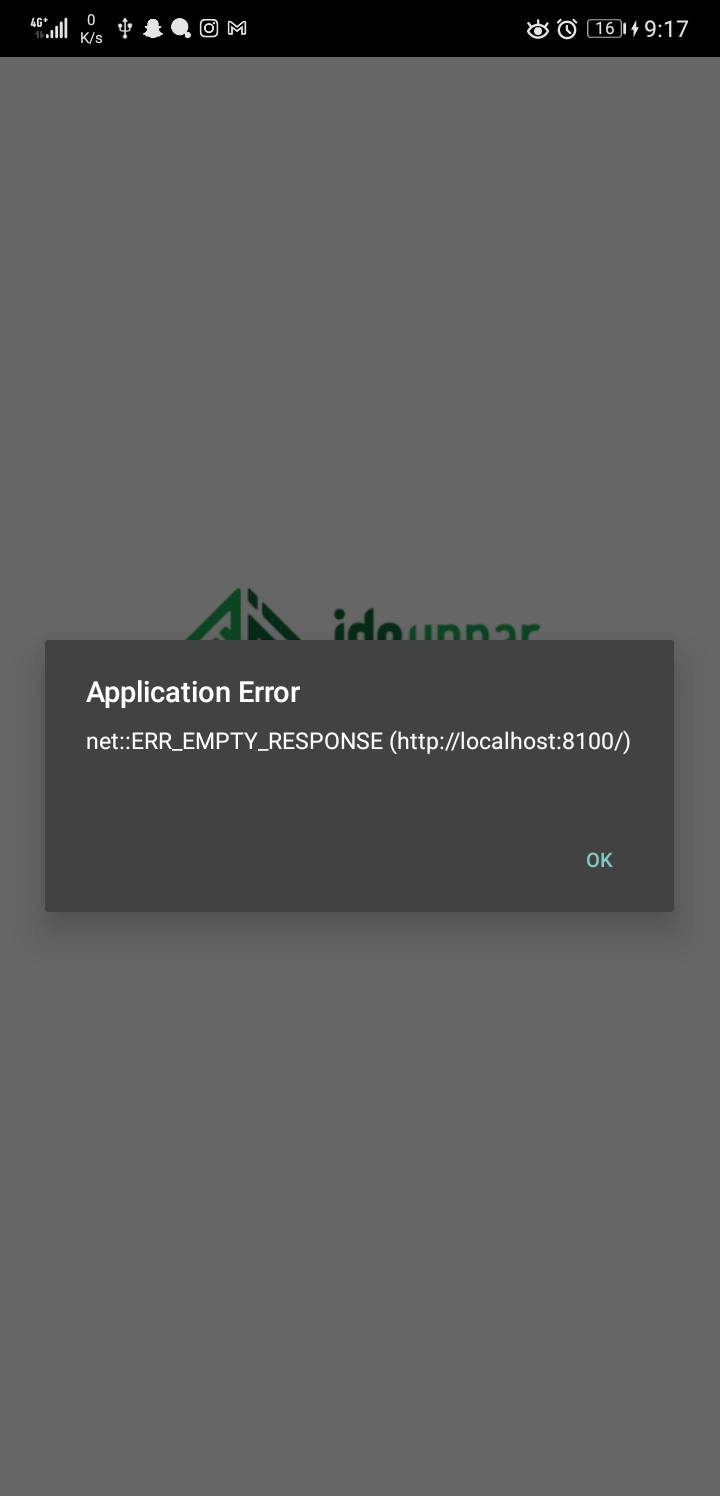
\includegraphics[scale=0.15]{no_connection-id.ac.unpar.moodlemobile.jpg}  
	\caption[\textit{Application error} dengan perintah \texttt{npm run dev:android}] {\textit{Application error} dengan perintah \texttt{npm run dev:android}} 
	\label{app:error:no-connection} 
\end{figure} 

Perintah \texttt{npx ionic cordova run android} akan menginstall \texttt{app-debug.apk} pada perangkat Android dan menajlankannya tanpa masalah. Ketika aplikasi berhasil berjalan pada perangkat bergerak, pengguna akan melalui halaman \textit{loading} seperti pada Gambar \ref{app:loading} kemudian diarahkan kehalaman \textit{login} di dalam aplikasi seperti pada Gambar \ref{app:login}.


\begin{figure}[H]
\begin{minipage}{.5\textwidth} 
	\centering  
	
\includegraphics[scale=0.14]{spalsh_screen-id.ac.unpar.moodlemobile.jpg}  
	\caption[Halaman \textit{loading} aplikasi] {Halaman \textit{loading} aplikasi} 
	\label{app:loading} 
\end{minipage}
\begin{minipage}{.5\textwidth}
	\centering  
	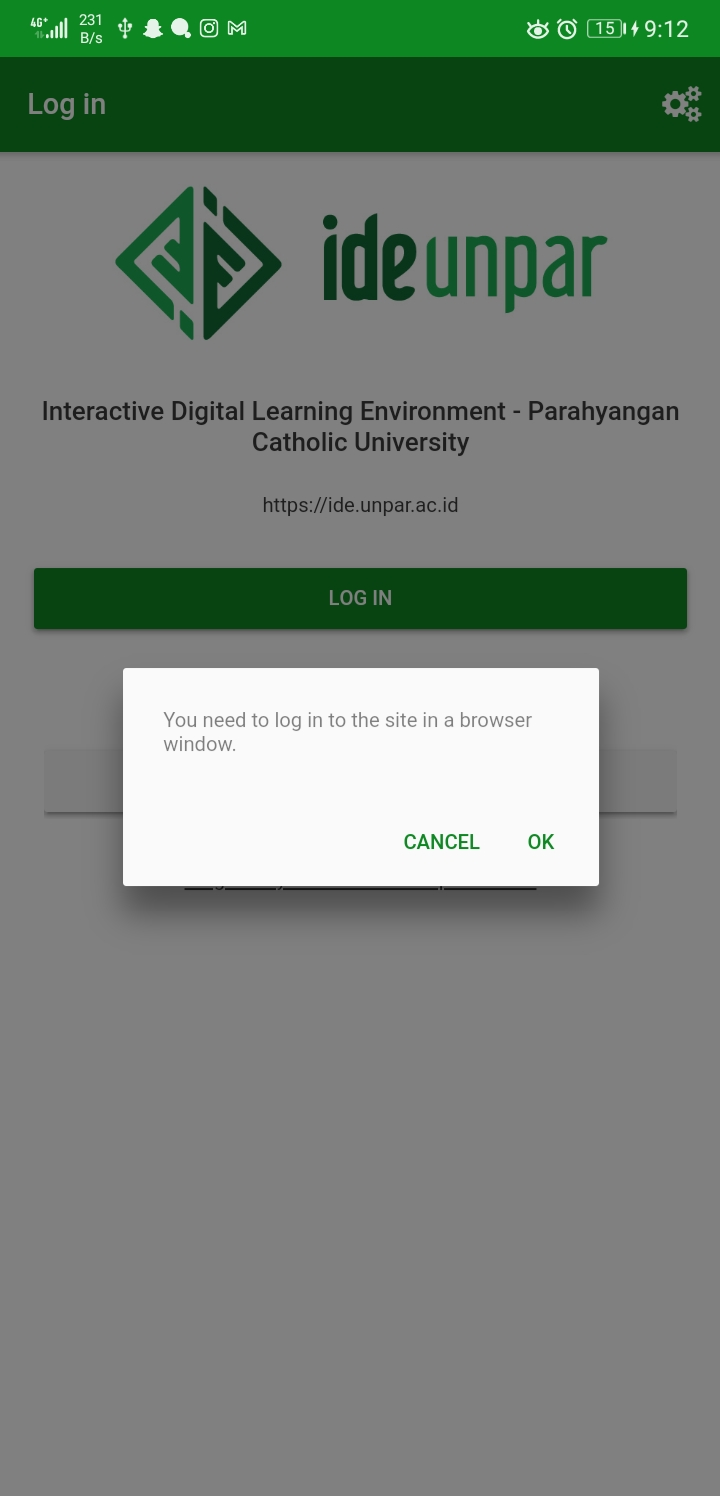
\includegraphics[scale=0.14]{login_screen-id.ac.unpar.moodlemobile.jpg}  
	\caption[Halaman \textit{login} aplikasi] {Halaman \textit{login} aplikasi} 
	\label{app:login} 
\end{minipage}
\end{figure}

Pengguna diharuskan menekan \textit{"OK"} pada \textit{pop-up} yang muncul untuk \textit{login} menggunakan SSO UNPAR. Ketika pengguna sudah berhasil \textit{login}. Pengguna akan diarahkan ke halaman \textit{Site Home} seperti pada Gambar \ref{app:site-home}, dimana isi halaman utama IDE UNPAR dapat diliahat. 

\begin{figure}[H] 
	\centering  
	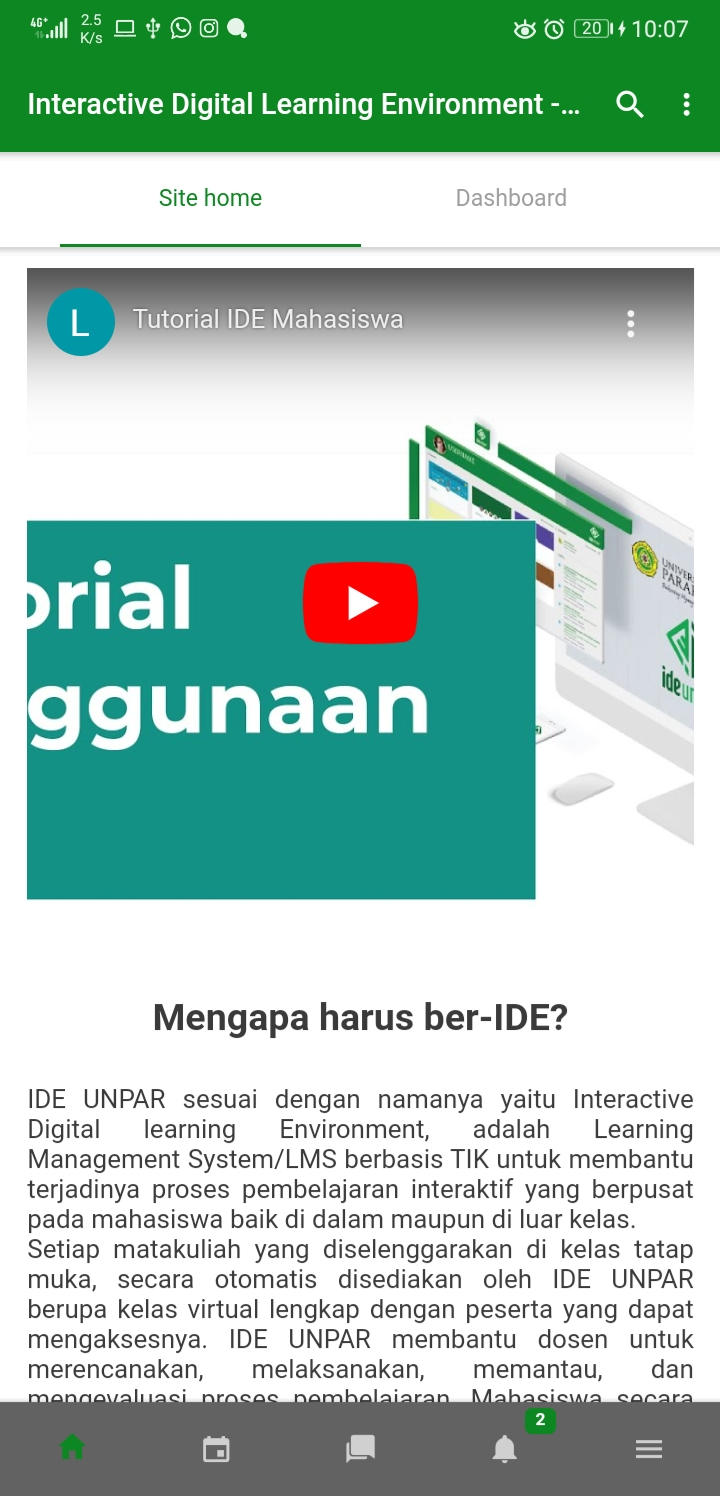
\includegraphics[scale=0.2]{site_home-id.ac.unpar.moodlemobile.jpg}  
	\caption[Halaman \textit{Site Home} aplikasi] {Halaman \textit{Site Home} aplikasi} 
	\label{app:site-home} 
\end{figure}  

Untuk melihat matakuliah yang diambil oleh pengguna, pengguna dapat menekan tombol \textit{"Dashboard"}. Pada bagian atas halaman \textit{Dashboard} pengguna dapat melihat \textit{course} atau mata kuliah yang baru diakses. Di bawah bagian \textit{Recently accessed courses} pengguna dapat melihat seluruh mata kuliah yang sedang diikuti dalam bagian \textit{Course overview}. Bagian \textit{Course overview} juga dapat diurutkan berdasarakan nama mata kuliah atau yang terakhir kali diakses oleh pengguna. Di bawah bagian \textit{Course overview} pengguna dapat melihat juga acara yang akan datang dan linimasa dari mata kuliah yang sedang ditempuh. Halaman \textit{Dashboard} dapat dilihat pada Gambar \ref{app:dashboard}

\begin{figure}[H]
	\centering  
	\begin{subfigure}[ht]{.3\textwidth}
	\centering
	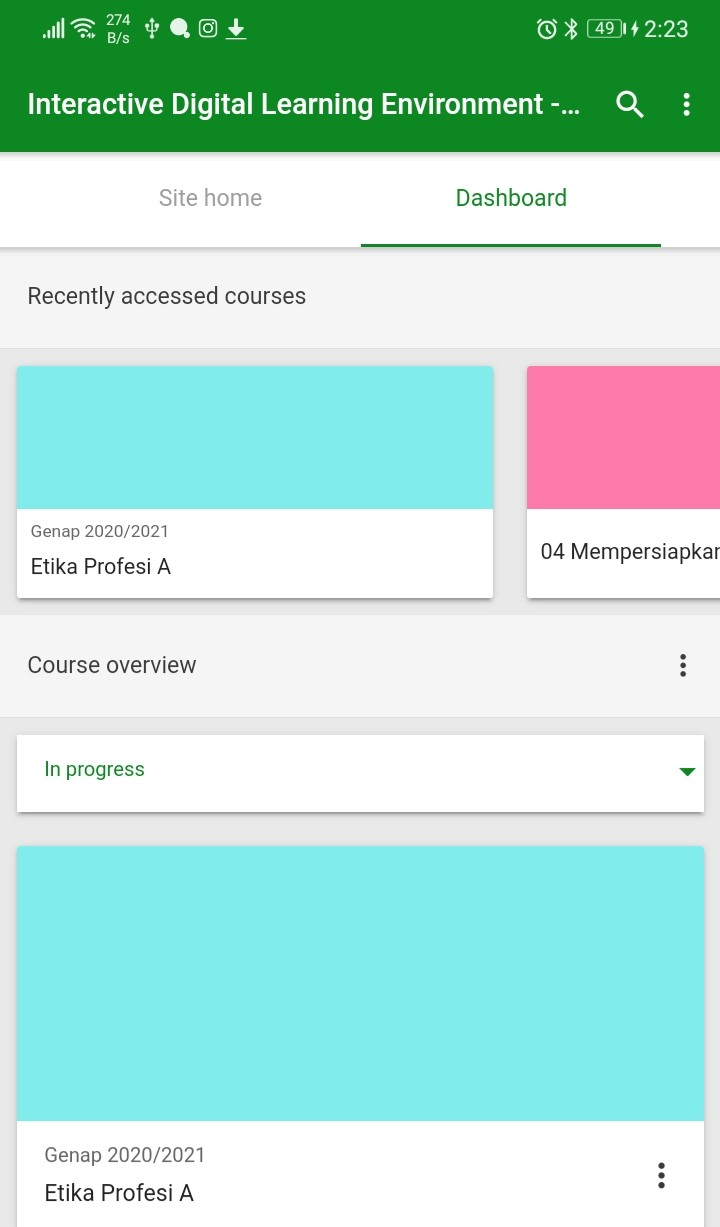
\includegraphics[scale=0.2]{dashboard-id.ac.unpar.moodlemobile-1.jpg} 
	\caption{Halaman \textit{Dashboard} sebelum di-\textit{scroll}}
	\end{subfigure}
	\hfill
	\begin{subfigure}[ht]{.3\textwidth}
	\centering
	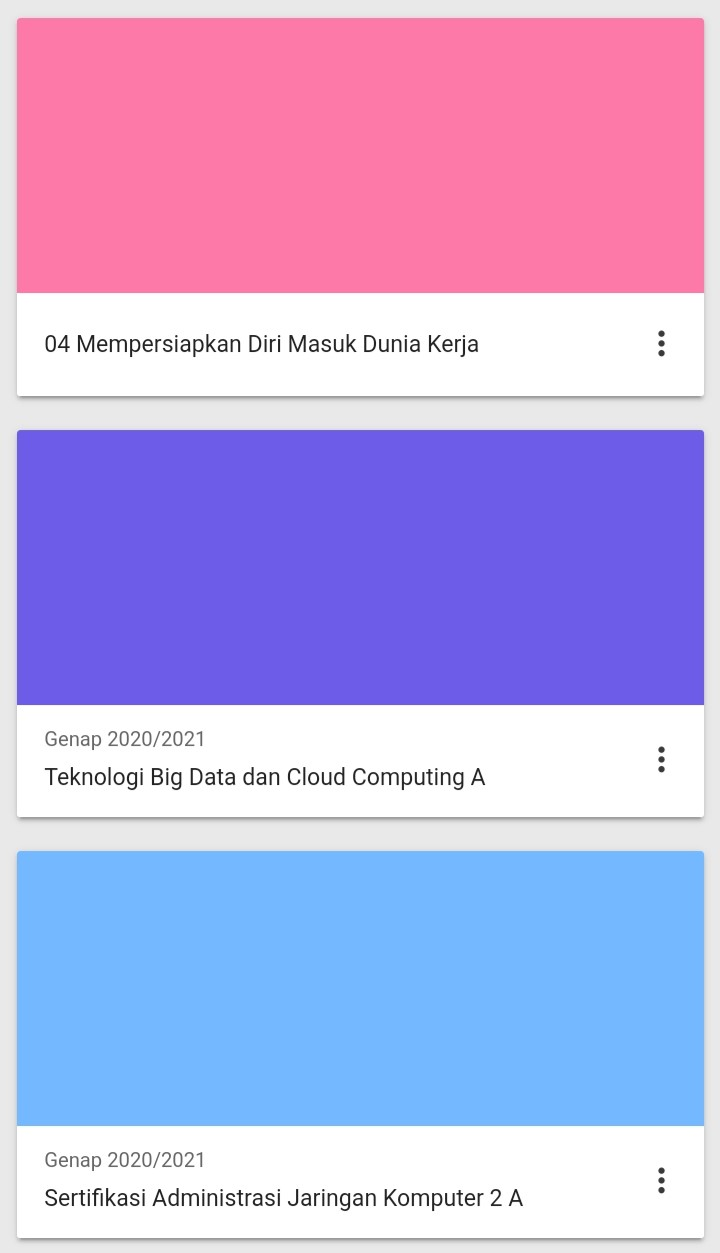
\includegraphics[scale=0.2]{dashboard-id.ac.unpar.moodlemobile-2.jpg} 
	\caption{Halaman \textit{Dashboard} setelah di-\textit{scroll}}
	\end{subfigure}
	\hfill
	\begin{subfigure}[ht]{.3\textwidth}
	\centering
	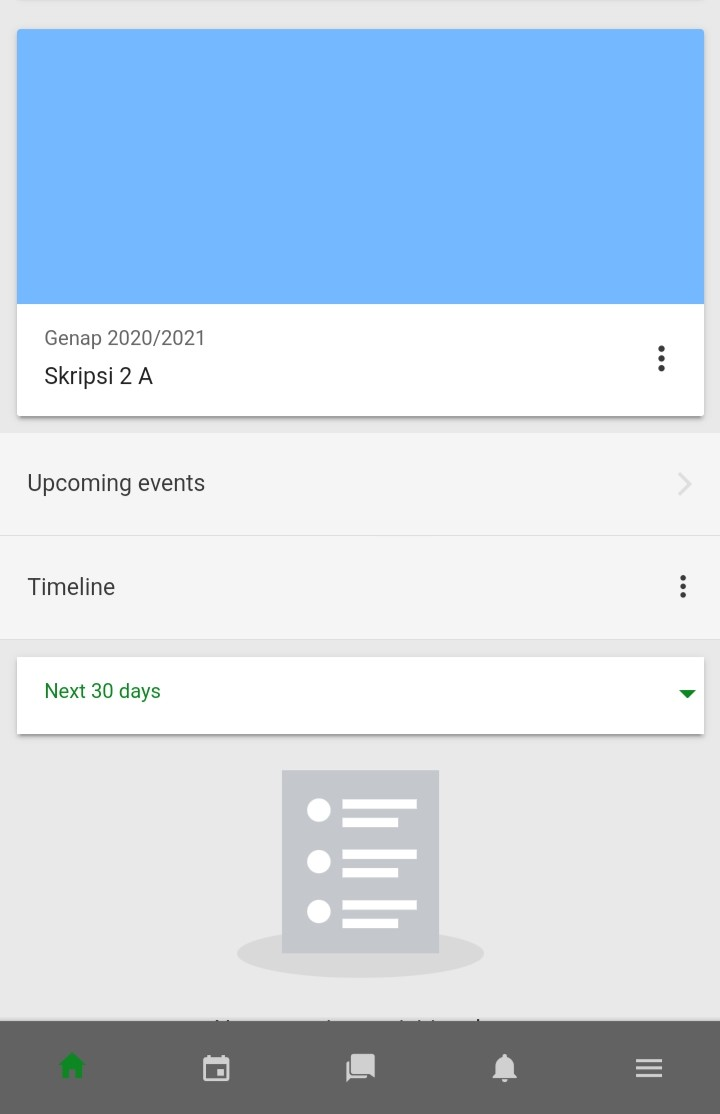
\includegraphics[scale=0.2]{dashboard-id.ac.unpar.moodlemobile-3.jpg} 
	\caption{Halaman \textit{Dashboard} setelah di-\textit{scroll}}
	\end{subfigure}

	\caption[Halaman \textit{Dashboard} aplikasi] {Halaman \textit{Dashboard} aplikasi} 
	\label{app:dashboard} 
\end{figure}  

\subsubsection{Halaman mata kuliah}

Halaman mata kuliah terbagi menjadi beberapa halaman yang akan menampilkan konten, peserta, nilai, dan kompentensi dari suatu mata kuliah. 
\begin{enumerate}
%\subsubsection{Halaman konten mata kuliah}
\item  \textbf{Halaman konten mata kuliah} \\
Halaman ini akan menunjukkan aktivitas yang terdapat didalam suatu mata kuliah yang telah disiapkan oleh dosen atau penyelenggara mata kuliah. Ketika pertama kali mengakses halaman ini, peserta akan dapat melihat seluruh konten, aktivitas, dan materi dari setiap topik mata kuliah yang dibuka seperti pada Gambar \ref{app:content}. Untuk melihat aktvitas berdasarakan setiap topik dari suatu mata kuliah pengguna dapat menekan tombol \textit{"All sections"} dan memilih topik yang ingin dilihat. Kemudian aplikasi akan memunculkan konten spesifik untuk topik mata kuliah yang dipilih seperti pada Gambar \ref{app:content:detail}.

\begin{figure}[H] 
	\centering 
	\begin{subfigure}[ht]{.3\textwidth}
	\centering
	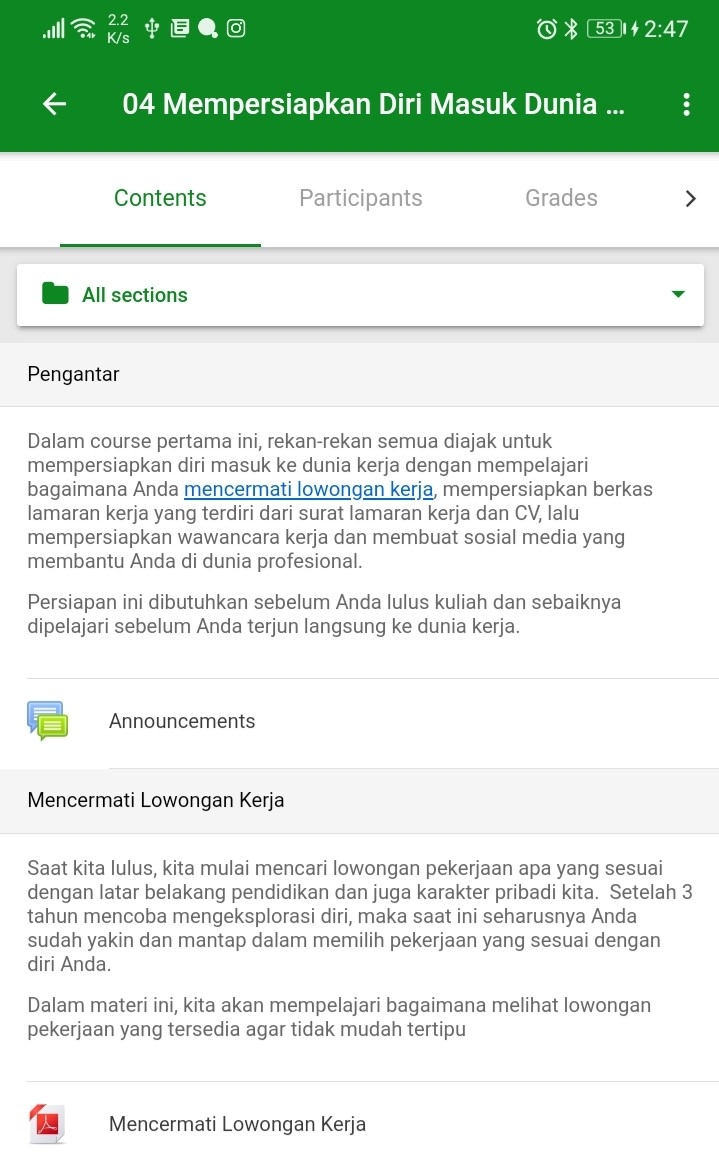
\includegraphics[scale=0.2]{course-content_id.ac.unpar.moodlemobile-1.jpg}  
	\caption{Halaman konten detail mata kuliah sebelum di-\textit{scroll}}
	\end{subfigure}
	\hfill
	\begin{subfigure}[ht]{.3\textwidth}
	\centering
	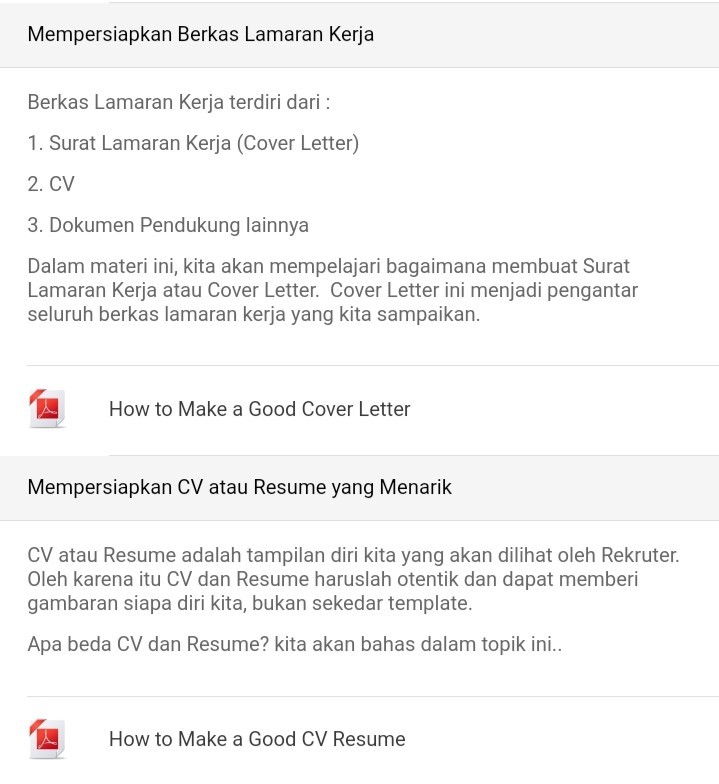
\includegraphics[scale=0.2]{course-content_id.ac.unpar.moodlemobile-2.jpg}  
	\caption{Halaman konten detail mata kuliah setelah di-\textit{scroll}}
	\end{subfigure}
	\hfill
	\begin{subfigure}[ht]{.3\textwidth}
	\centering
	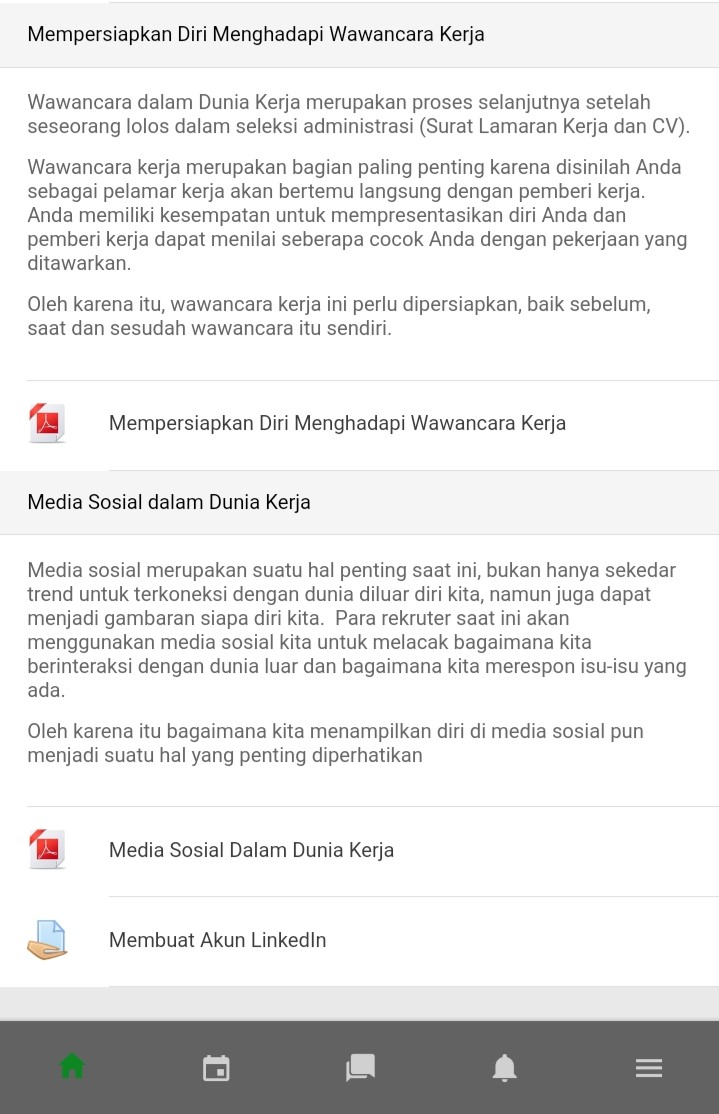
\includegraphics[scale=0.2]{course-content_id.ac.unpar.moodlemobile-3.jpg}  
	\caption{Halamankonten detail mata kuliah setelah di-\textit{scroll}}
	\end{subfigure} 
	\caption[Halaman konten detail mata kuliah aplikasi] {Halaman konten detail mata kuliah aplikasi} 
	\label{app:content} 
\end{figure}  

\begin{figure}[H] 
	\centering  
	\includegraphics[scale=0.15]{course-content-detail_id.ac.unpar.moodlemobile.jpg}  
	\caption[Halaman konten detail mata kuliah aplikasi] {Halaman konten detail mata kuliah aplikasi} 
	\label{app:content:detail} 
\end{figure}  

%\subsubsection{Halaman peserta mata kuliah}
\item \textbf{Halaman peserta mata kuliah} \\
Halaman ini menunjukkan pengajar dan siswa yang mengikuti mata kuliah yang dipilih seperti pada Gambar \ref{app:participants}. Pada halaman ini pengguna juga dapat mencari nama peserta mata kuliah dan melihat profil dari peserta mata kuliah. Namun mahasiswa pengguna hanya dapat melihat peserta dengan peran \textit{teacher}. 

\begin{figure}[H] 
	\centering  
	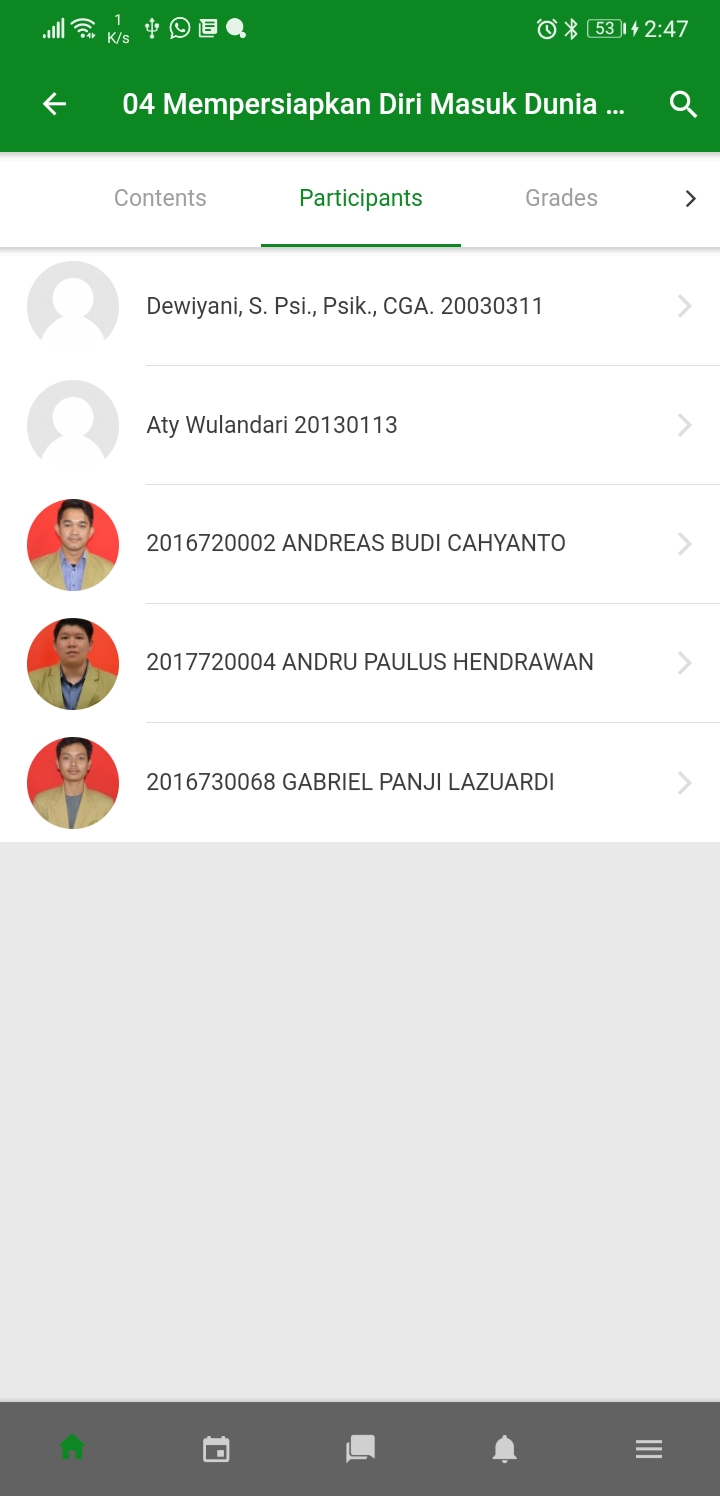
\includegraphics[scale=0.15]{course-participant_id.ac.unpar.moodlemobile.jpg}  
	\caption[Halaman \textit{Participants} aplikasi] {Halaman \textit{Participants} aplikasi} 
	\label{app:participants} 
\end{figure}  

%\subsubsection{Halaman nilai matakuliah}
\item \textbf{Halaman nilai mata kuliah} \\
Halaman ini akan menunjukkan nilai tugas dan nilai total mata kuliah pengguna. Halaman nilai dapat dilihat pada Gambar \ref{app:grades}.

\begin{figure}[H] 
	\centering  
	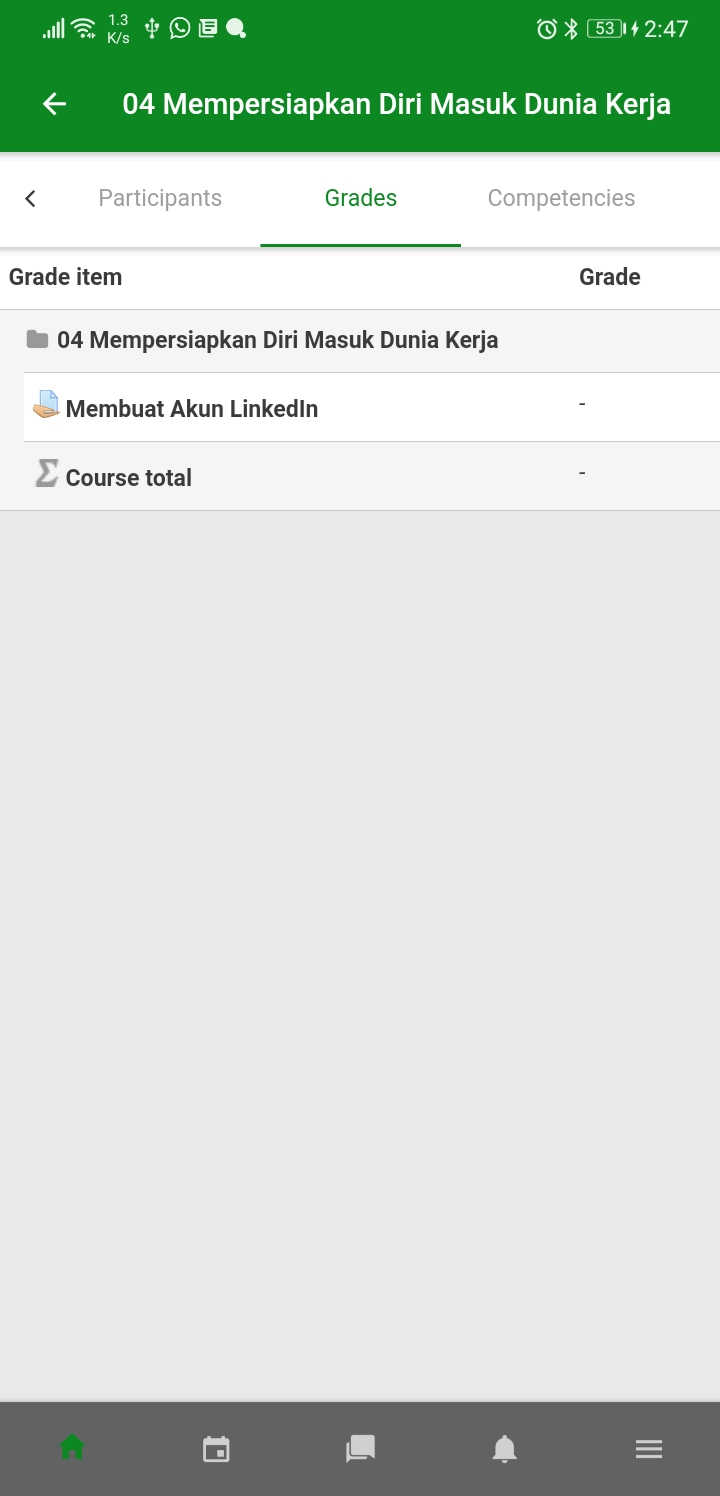
\includegraphics[scale=0.15]{course-grades_id.ac.unpar.moodlemobile.jpg}  
	\caption[Halaman \textit{Grades} aplikasi] {Halaman \textit{Grades} aplikasi} 
	\label{app:grades} 
\end{figure}  

%\subsubsection{Halaman kompentensi mata kuliah}

\item \textbf{Halaman kompetensi mata kuliah} \\
Halaman ini menunjukkan kompentensi pengguna pada mata kuliah yang sedang diambil. Karena tidak ada kompentensi yang dihubungkan dari mata kuliah yang sedang ditempuh peneliti maka halaman \textit{Competencies} akan kosong. Halaman \textit{Competencies} dapat dilihat pada Gambar \ref{app:competencies}.

\begin{figure}[H] 
	\centering  
	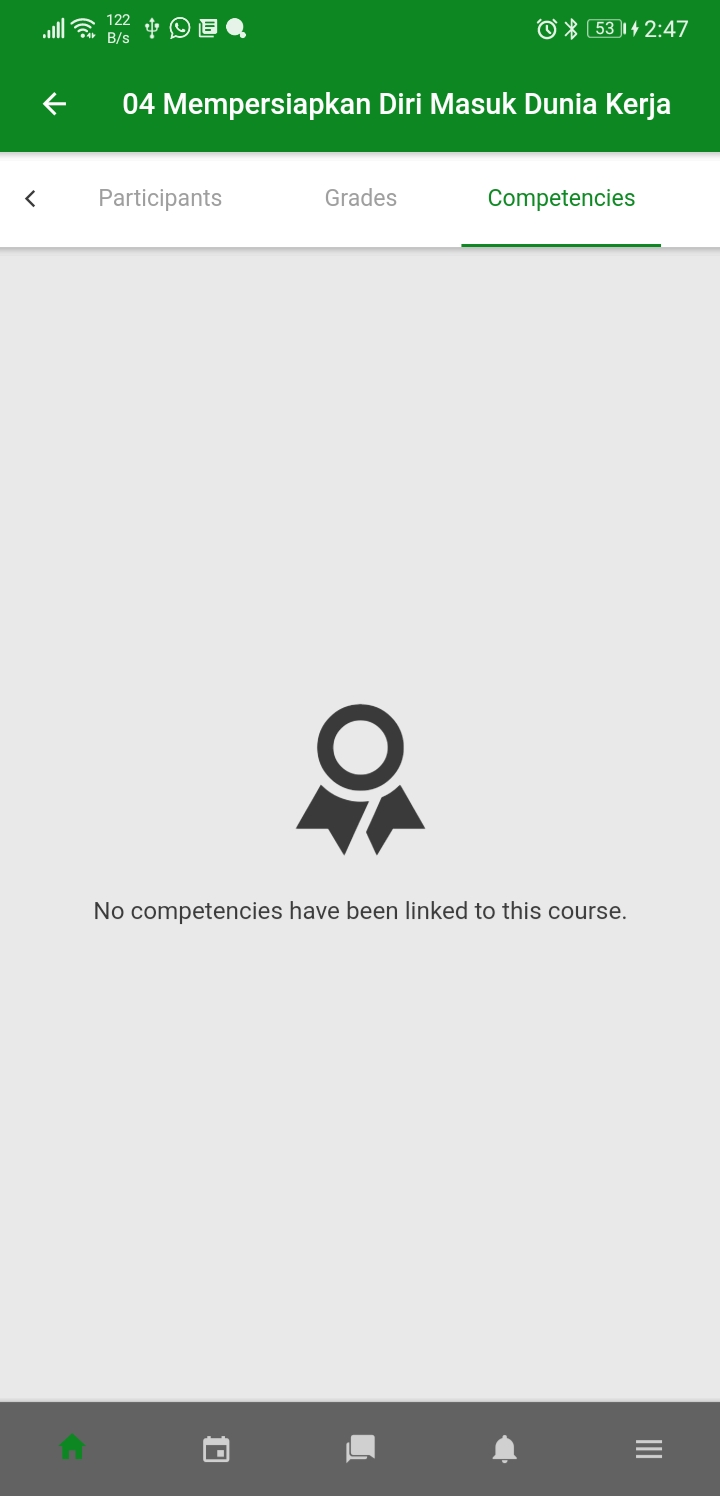
\includegraphics[scale=0.15]{course-compentencies_id.ac.unpar.moodlemobile.jpg}  
	\caption[Halaman \textit{Competencies} aplikasi] {Halaman \textit{Competencies} aplikasi} 
	\label{app:competencies} 
\end{figure}  

\end{enumerate}

\subsubsection{Halaman \textit{Calendar events}}

Halaman \textit{Calendar events} dapat diakses melalui \textit{navigation bar} dengan menekan ikon kalender. Pada halaman ini pengguna akan dapat melihat kapan saja tenggat waktu suatu tugas, kapan adanya kuis, dan aktivitas lain yang telah ditentukan oleh penyelenggara mata kuliah selama penyelenggara menetukan tanggal-tanggalnya. Halaman \textit{Calendar events} dapat dilihat pada Gambar \ref{app:calendar}.

\begin{figure}[H] 
	\centering  
	\includegraphics[scale=0.15]{Calendar_id.ac.unpar.moodlemobile.jpg}  
	\caption[Halaman \textit{Calendar events} aplikasi] {Halaman \textit{Calendar events} aplikasi} 
	\label{app:calendar} 
\end{figure}  

\subsubsection{Halaman \textit{Messages}}

Halaman \textit{Messages} dapat diakses dengan menekan ikon \textit{chat box} pada \textit{navigation bar} aplikasi. Ketika dibuka halaman ini akan menunjukkan menu kontak, bagian \textit{starred} untuk pesan yang ditandai dengan bintang, bagian \textit{group} untuk pesan dari kelompok dari mata kuliah yang diikuti, dan \textit{private} untuk pesan yang dikirim ke pengguna dari pengguna lain. Halaman \textit{Messages} dapat dilihat pada Gambar \ref{app:messages}.


\begin{figure}[H] 
	\centering  
	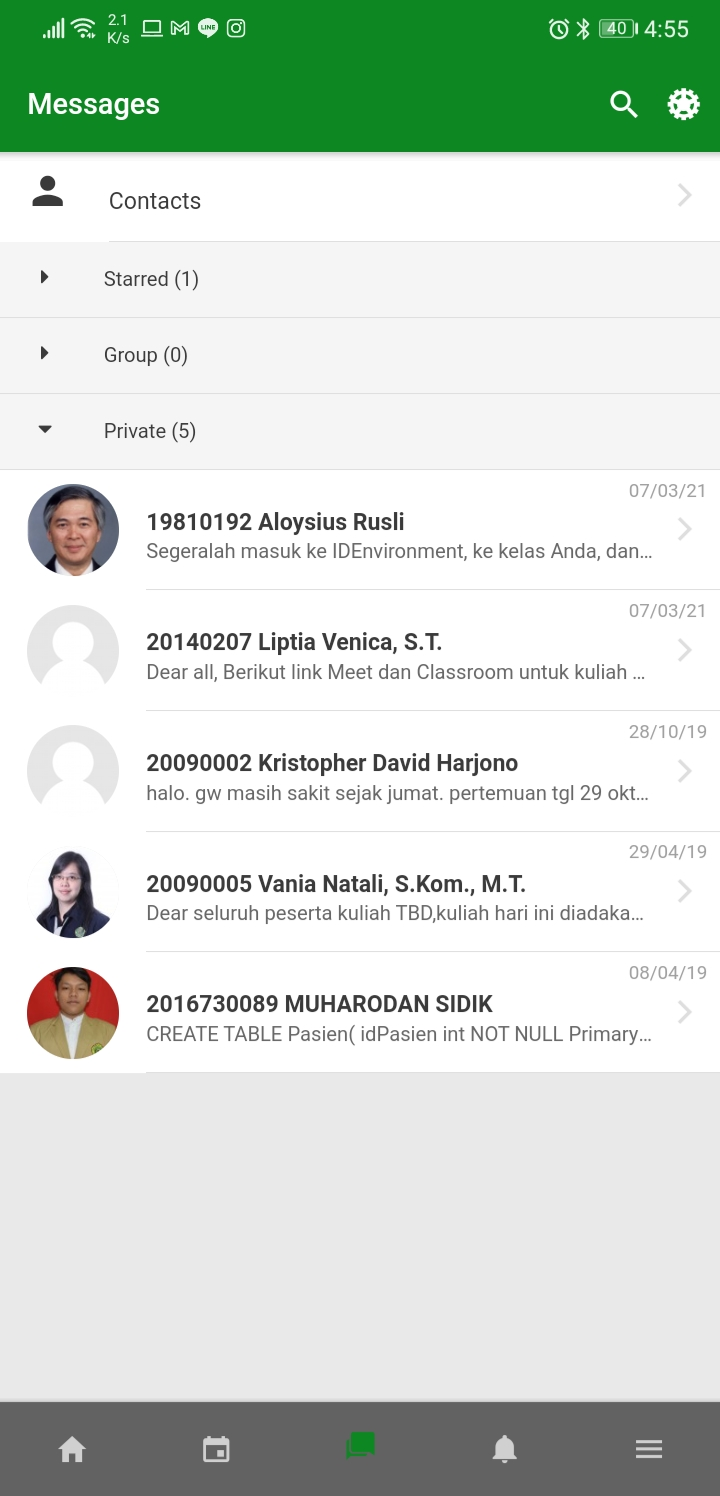
\includegraphics[scale=0.15]{message-private_id.ac.unpar.moodlemobile.jpg}  
	\caption[Halaman \textit{Messages} aplikasi] {Halaman \textit{Messages} aplikasi} 
	\label{app:messages} 
\end{figure}  

Melihat kontak pengguna dapat dikases dengan menekan menu \textit{Contacts} pada halaman \textit{Messages}. Pada halaman \textit{Contacts} pengguna akan dapat melihat kontaknya yang terdaftar seperti pada Gambar \ref{app:messages:contact} dan melihat permintaan kontak dari pengguna lain seperti pada Gambar \ref{app:messages:request}.

\begin{figure}[H]
\centering
\begin{minipage}{.3\textwidth} 
	\centering  
	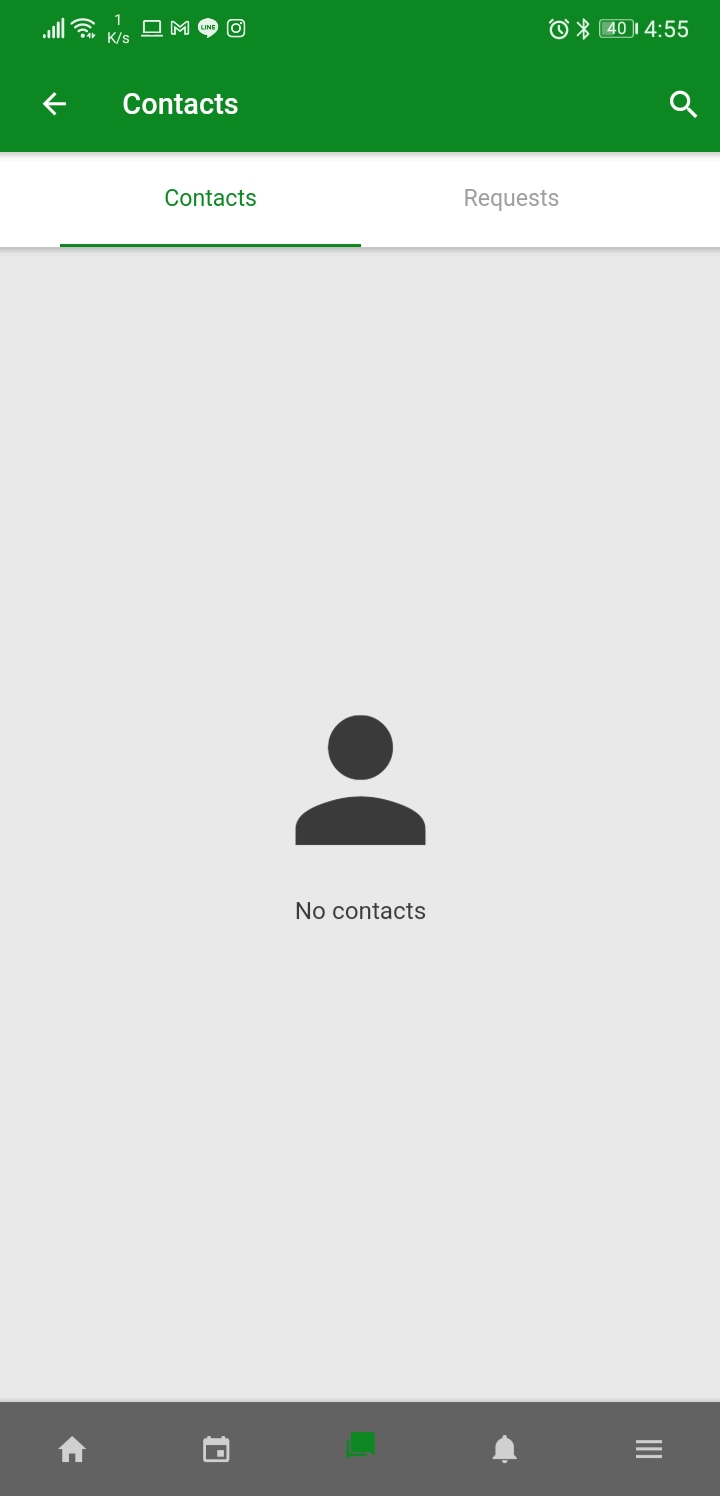
\includegraphics[scale=0.13]{messages-contact_id.ac.unpar.moodlemobile.jpg}  
	\caption[Halaman \textit{Contact} aplikasi] {Halaman \textit{Contact} aplikasi} 
	\label{app:messages:contact} 
\end{minipage}
\hspace{.2\textwidth}
\begin{minipage}{.3\textwidth}
	\centering  
	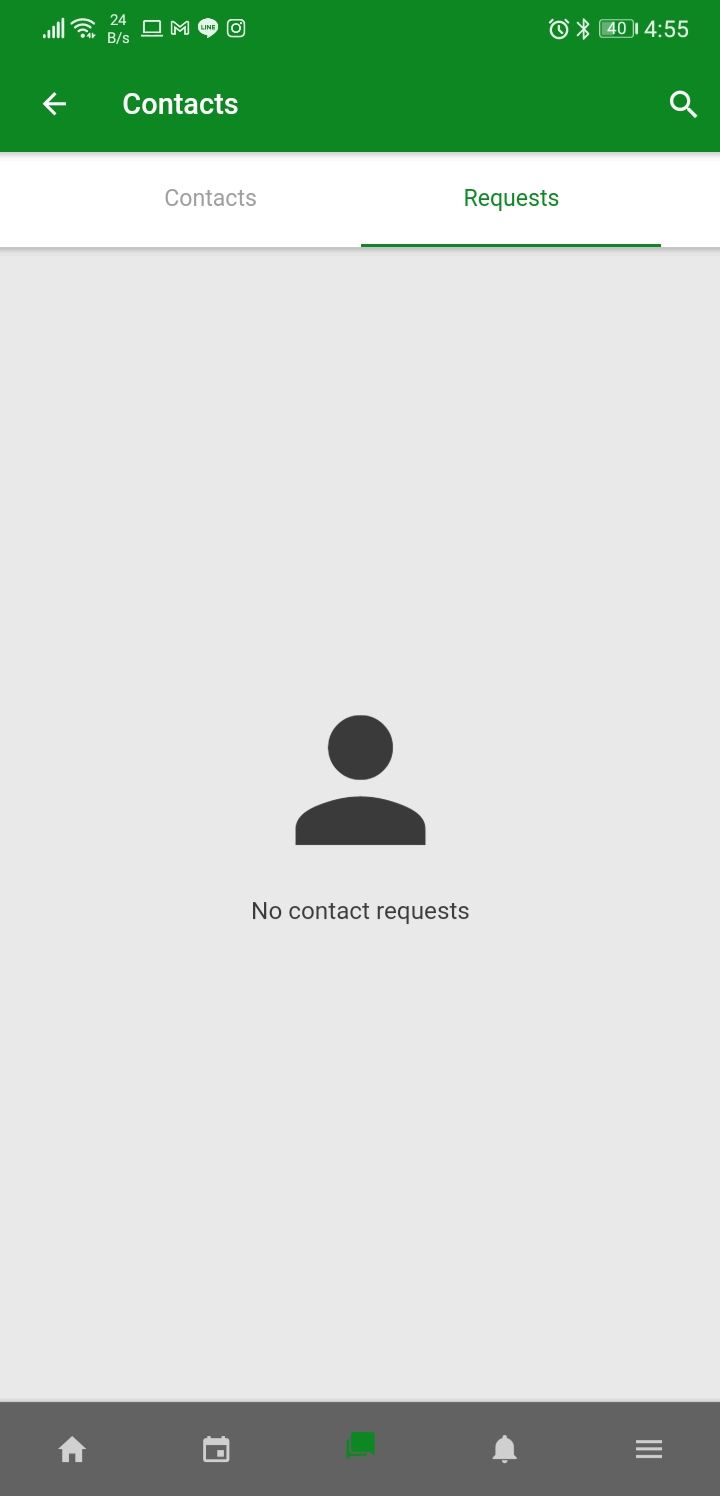
\includegraphics[scale=0.13]{messages-request_id.ac.unpar.moodlemobile.jpg}  
	\caption[Halaman permintaan kontak aplikasi] {Halaman permintaan kontak aplikasi} 
	\label{app:messages:request} 
\end{minipage}
\end{figure}

\subsubsection{Halaman \textit{Notifications}}

Halaman ini akan menunjukkan seluruh notifikasi yang diterima oleh pengguna, baik notfikassi tenggat waktu suatu tugas ataupun pesan dari pengguna lain. Halaman \textit{Notifications} dapat diakses dengan menekan ikon lonceng pada \textit{navgiation bar} aplikasi. Halaman \textit{Notification} dapat dilihat pada Gambar \ref{app:notifications}.


\begin{figure}[H] 
	\centering  
	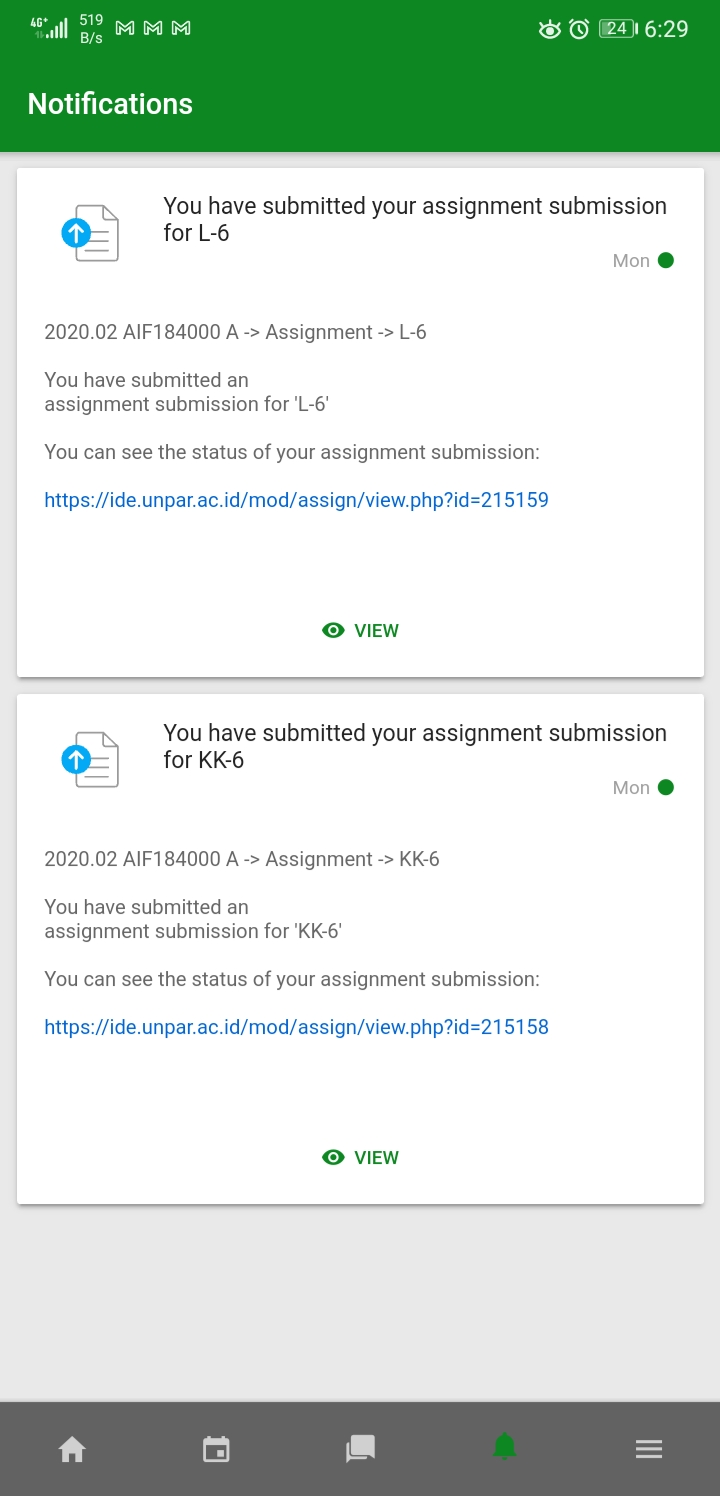
\includegraphics[scale=0.15]{notifications_id.ac.unpar.moodlemobile.jpg}  
	\caption[Halaman \textit{Notifications} aplikasi] {Halaman \textit{Notifications} aplikasi} 
	\label{app:notifications} 
\end{figure}  

\subsubsection{Halaman menu}

Halaman ini berisi menu-menu yang dapat digunakan pengguna untuk mengakses halama-halaman lain pada aplikasi. Halaman ini dapat dikases dengan menekan ikon tiga garis horisontal pada \textit{navigation bar} aplikasi. Tampilan halaman menu dapat dilihat pada Gambar \ref{app:menu}.

Halaman menu mengandung beberapa menu lain seperti \textit{Grades}, \textit{Files}, \textit{Scan QR code}, \textit{Website}, Student Portal UNPAR, \textit{Help}, \textit{Perferences}, dan \textit{App settings}.

\begin{figure}[H] 
	\centering  
	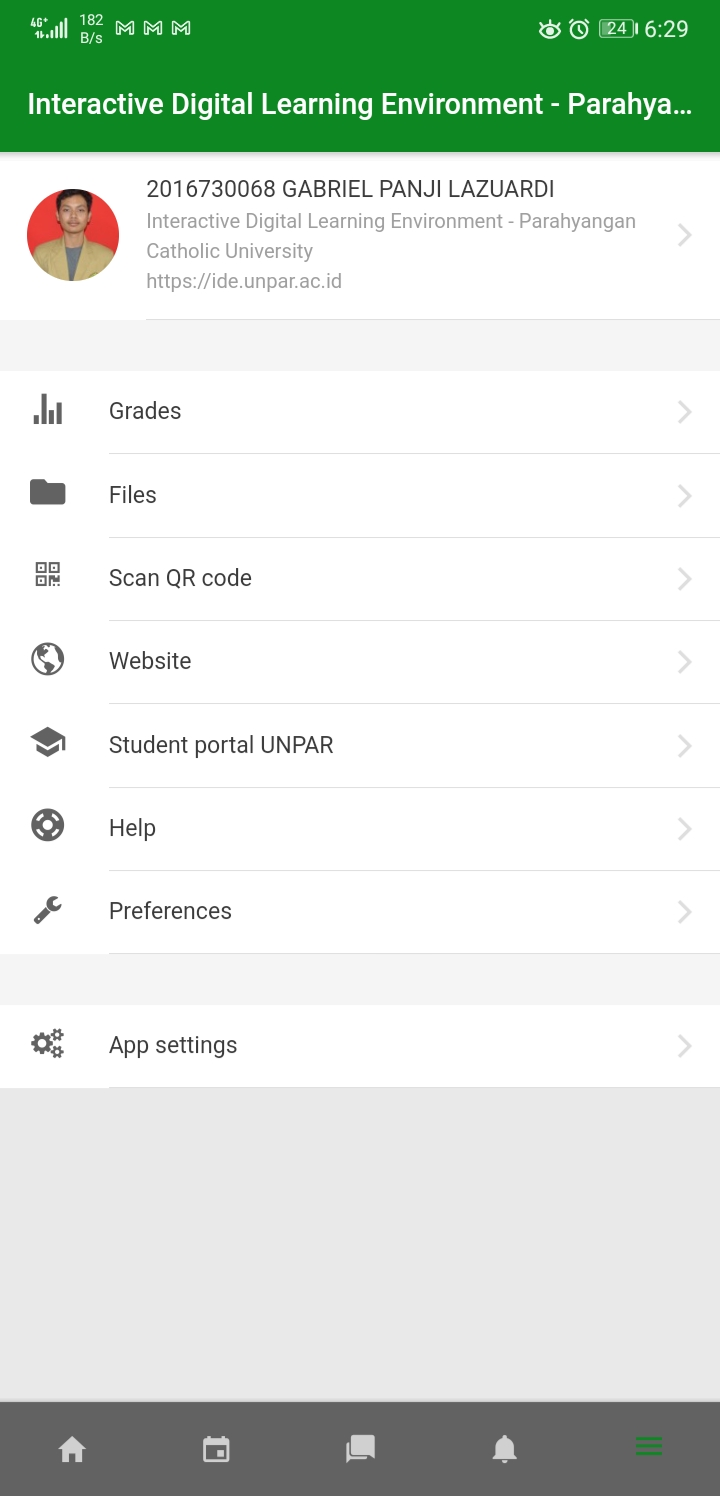
\includegraphics[scale=0.15]{menu_id.ac.unpar.moodlemobile.jpg}  
	\caption[Halaman menu aplikasi] {Halaman menu aplikasi} 
	\label{app:menu} 
\end{figure}  

\begin{enumerate}
%\subsubsection{Menu \textit{Grades}}
\item \textbf{Menu \textit{Grades}} \\
Menu \textit{Grades} akan mengarahkan pengguna menuju halaman \textit{Grades} yang akan menunjukkan mata kuliah yang diambil oleh pengguna beserta dengan total nilainya. Ketika satu nama mata kuliah dipilih, maka pengguna akan diarahkan ke halaman detail niali dari mata kuliah tersebut. Halaman \textit{Grades} dapat dilihat pada Gambar \ref{app:menu:grades}.

\begin{figure}[H] 
	\centering  
	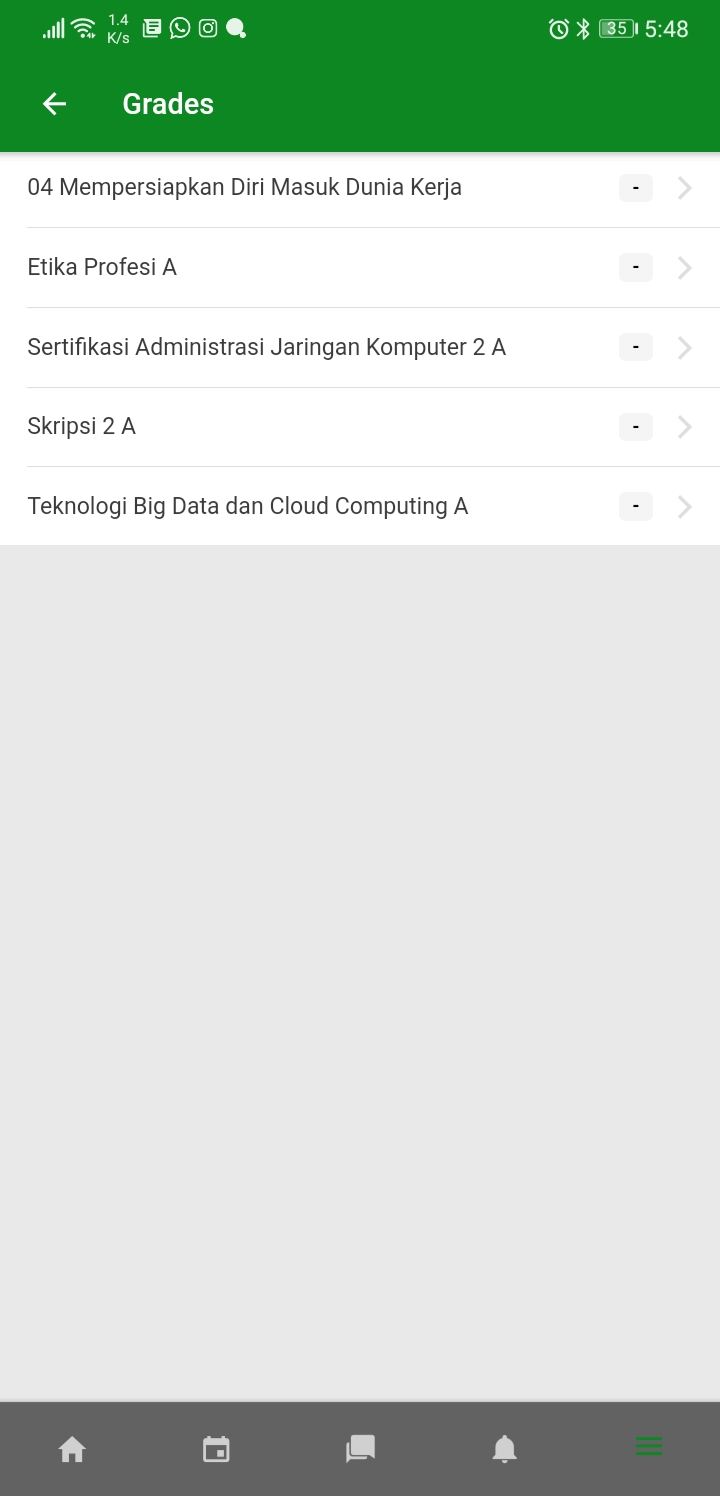
\includegraphics[scale=0.15]{menu-grades_id.ac.unpar.moodlemobile.jpg}  
	\caption[Halaman menu \textit{Grades} aplikasi] {Halaman menu \textit{Grades} aplikasi} 
	\label{app:menu:grades} 
\end{figure}  

%\subsubsection{Menu \textit{Files}}
\item \textbf{Menu \textit{Files}} \\

Menu ini akan mengarahkan pengguna ke halaman \textit{Files}. Ketika halaman tersebut pertama kali dibuka, pengguna dapat melihat file-file pribadinya yang tersimpan pada server IDE UNPAR. Dapat dilihat pada Gambar \ref{app:menu:files:private}. Dari halaman tersebut pengguna dapat menambahkan file-file dengan menekan tombol dengan ikon tanda tambah.


\begin{figure}[H] 
	\centering  
	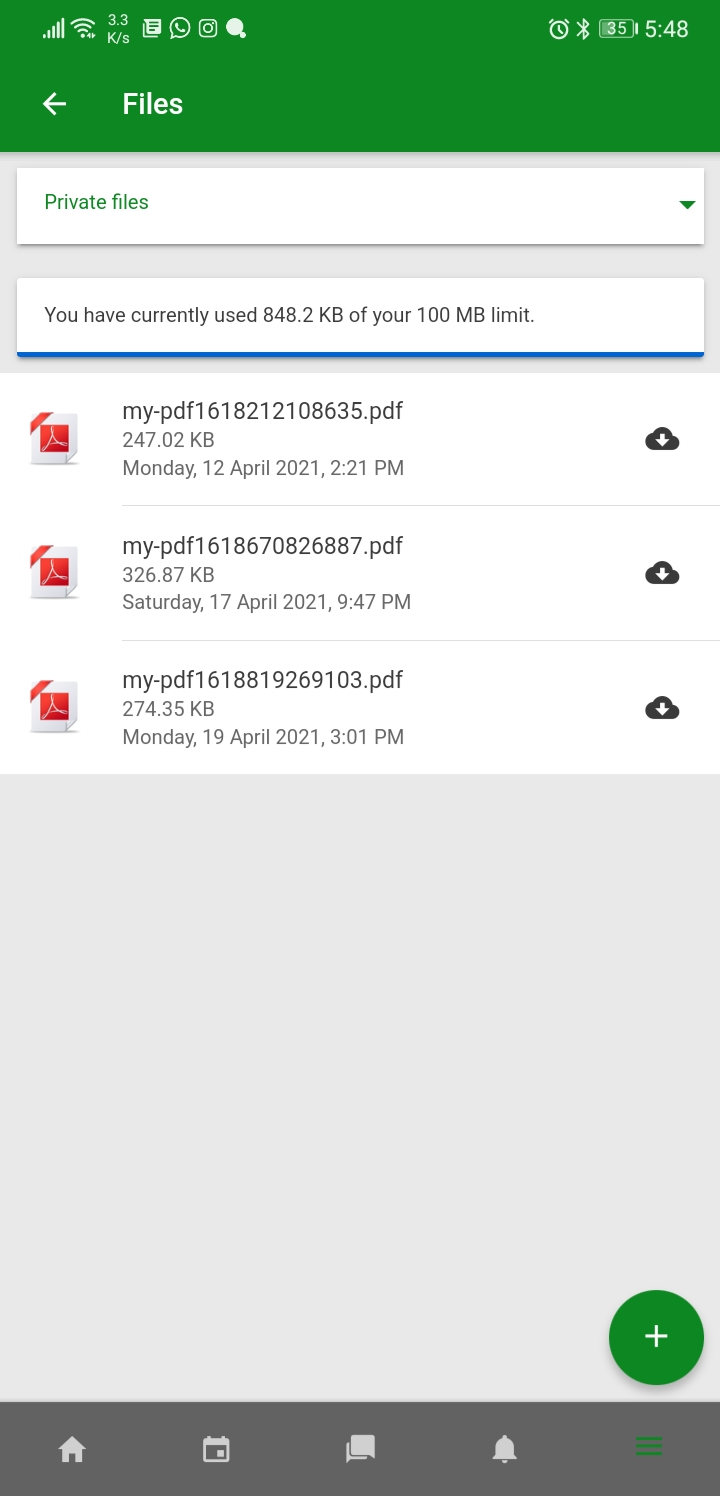
\includegraphics[scale=0.15]{menu-files-private_id.ac.unpar.moodlemobile.jpg}  
	\caption[Halaman menu \textit{Files} aplikasi] {Halaman menu \textit{Files} aplikasi} 
	\label{app:menu:files:private} 
\end{figure}  

 Pengguna juga dapat melihat file-file public dengan menekan \textit{dropdown} yang berada dibawah \textit{header} dan memilih site files. Halaman \textit{Site files} dapat dilihat pada Gambar \ref{app:menu:files:site}

\begin{figure}[H] 
	\centering  
	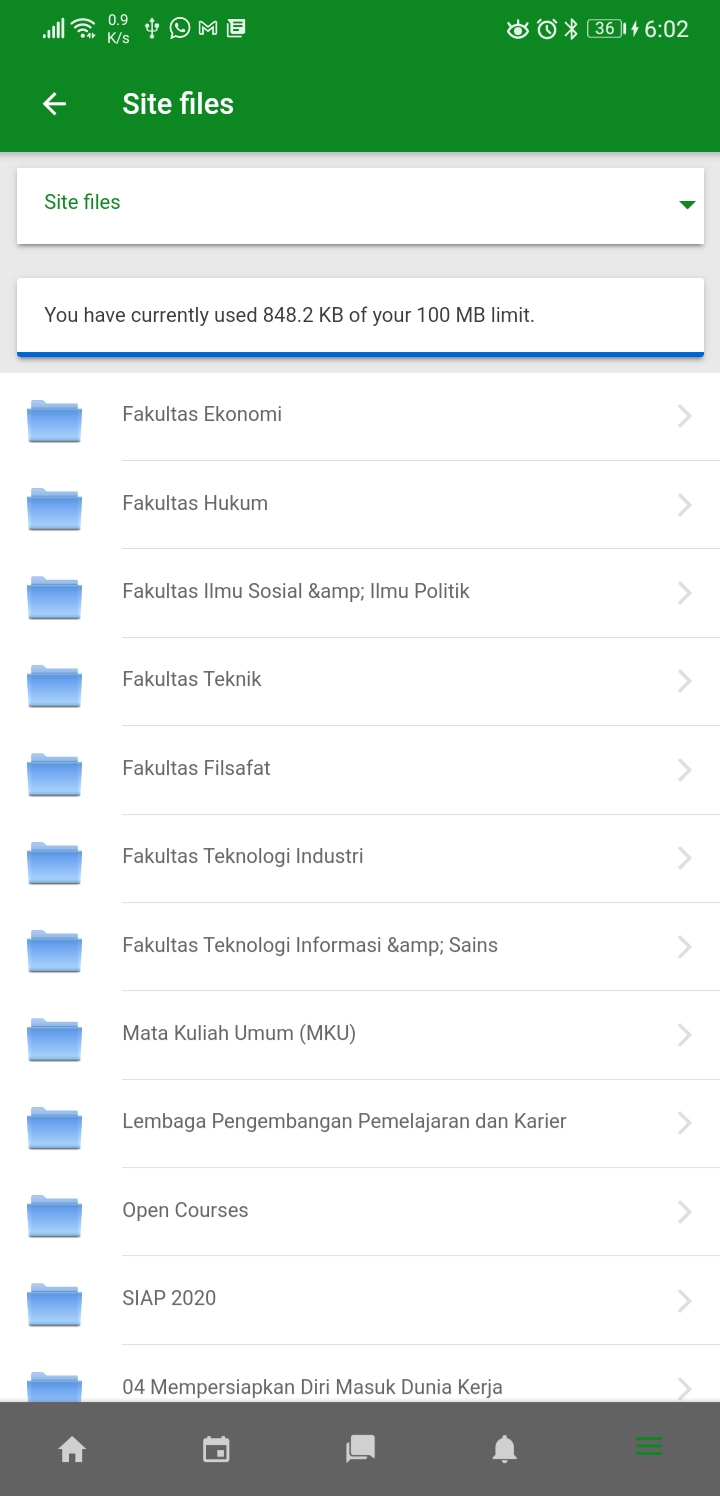
\includegraphics[scale=0.15]{menu-files-site_id.ac.unpar.moodlemobile.jpg}  
	\caption[Halaman menu \textit{Site files} aplikasi] {Halaman menu \textit{Site files} aplikasi} 
	\label{app:menu:files:site} 
\end{figure}  

%\subsubsection{Menu \textit{Scan QR}}
\item \textbf{Menu \textit{Scan QR}} \\
Menu ini akan membuka kamera dari perangkat pengguna untuk memindai kode QR dari Moodle.

%\subsubsection{Menu Website}
\item \textbf{Menu \textit{Website}} \\
Menu ini akan mengarahkan pengguna ke situs IDE UNPAR, dengan membuka halaman tersebut pada \textit{browser} perangkat pengguna.

%\subsubsection{Menu Student Portal UNPAR}
\item \textbf{Menu Student Portal UNPAR} \\
Menu ini akan mengarahkan pengguna ke situs Student Portal UNPAR, dengan membuka halaman tersebut pada \textit{browser} perangkat pengguna.

%\subsubsection{Menu \textit{Help}}
\item \textbf{Menu \textit{Help}} \\
Menu ini akan mengarahkan pengguna ke tautan \url{http://docs.moodle.org/38/en/Moodle\_app}. Tautan tersebut berisi bantuan cara penggunaan aplikasi Moodle mobile.

%\subsubsection{Menu \textit{Perferences}}
\item \textbf{Menu \textit{Perferences}} \\
Menu ini akan mengarahkan pengguna ke halaman \textit{Perferences} yang berisi pengaturan untuk fitur \textit{messages} dan \textit{notifications}. Selain itu di halaman \textit{Perferences} pengguna dapat membebaskan tempat penyimpanan yang digunakan oleh aplikasi dan mensinkronisasikan aplikasi dengan situs IDE UNPAR.

\item \textbf{Menu \textit{Change Site}} \\
Menu ini awalnya berguna untuk pengguna menambahkan situs yang terhubung dengan aplikasi Moodle mobile, menambahkan profil pengguna di dalam aplikasi, dan untuk \textit{logout}. Namun karena aplikasi IDE UNPAR mobile sudah di-\textit{hardcode} untuk mengarah langsung ke situs IDE UNPAR maka fitur ini hanya berfungsi untuk \textit{logout} dengan menekan ikon pensil kemudia menekan ikon tempat sampah pada sisi kanan profil dan menambahkan profil pengguna dengan menekan tombol ikon tanda tambah. Halaman \textit{Change Site} dapat dilihat pada Gambar \ref{app:menu:change:sites}.

\begin{figure}[H] 
	\centering  
	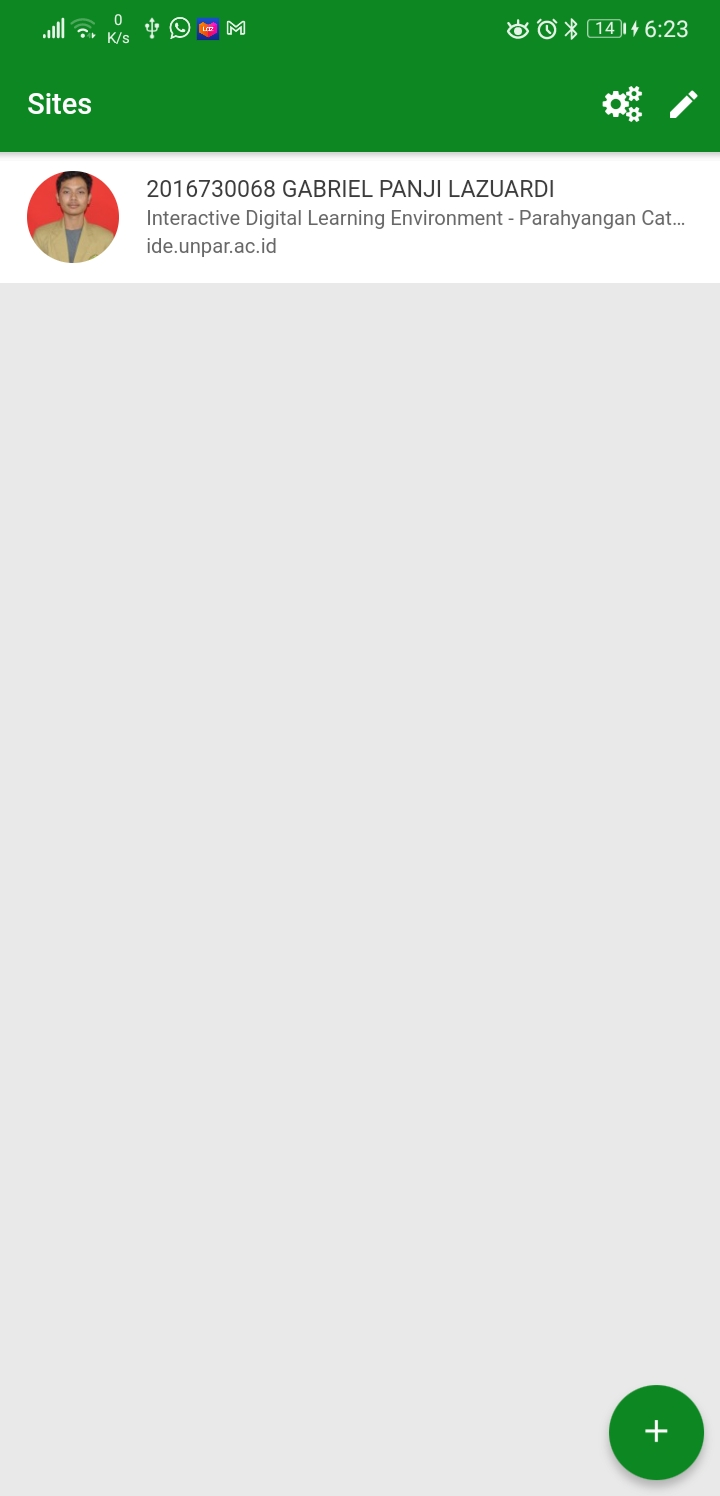
\includegraphics[scale=0.15]{menu-change-site_id.ac.unpar.moodlemobile.jpg}  
	\caption[Halaman menu \textit{Change Sites}] {Halaman menu \textit{Change Sites}} 
	\label{app:menu:change:sites} 
\end{figure}  

%\subsubsection{Menu \textit{App settings}}
\item \textbf{Menu \textit{App settings}} \\
Menu ini akan mengarahkan pengguna ke halaman \textit{App settings}, dimana pengguna dapat mengatur pengaturan umum aplikasi, pengguna ruang penyimpanan aplikasi, sinkronisasi aplikasi, dan melihat informasi tentang aplikasi.
\end{enumerate}


\subsubsection{Pengujian fitur \textit{Scan PDF}}

Fitur \textit{Scan PDF} dapat dikases melalui menu kemudian dengan memilih \textit{Files}. Dari halaman \textit{Files}, pengguna dapat menekan tombol dengan ikon tanda tambah untuk melihat pilihan cara mengunggah file seperti pada Gambar \ref{app:menu:files:options}. 

\begin{figure}[H] 
	\centering  
	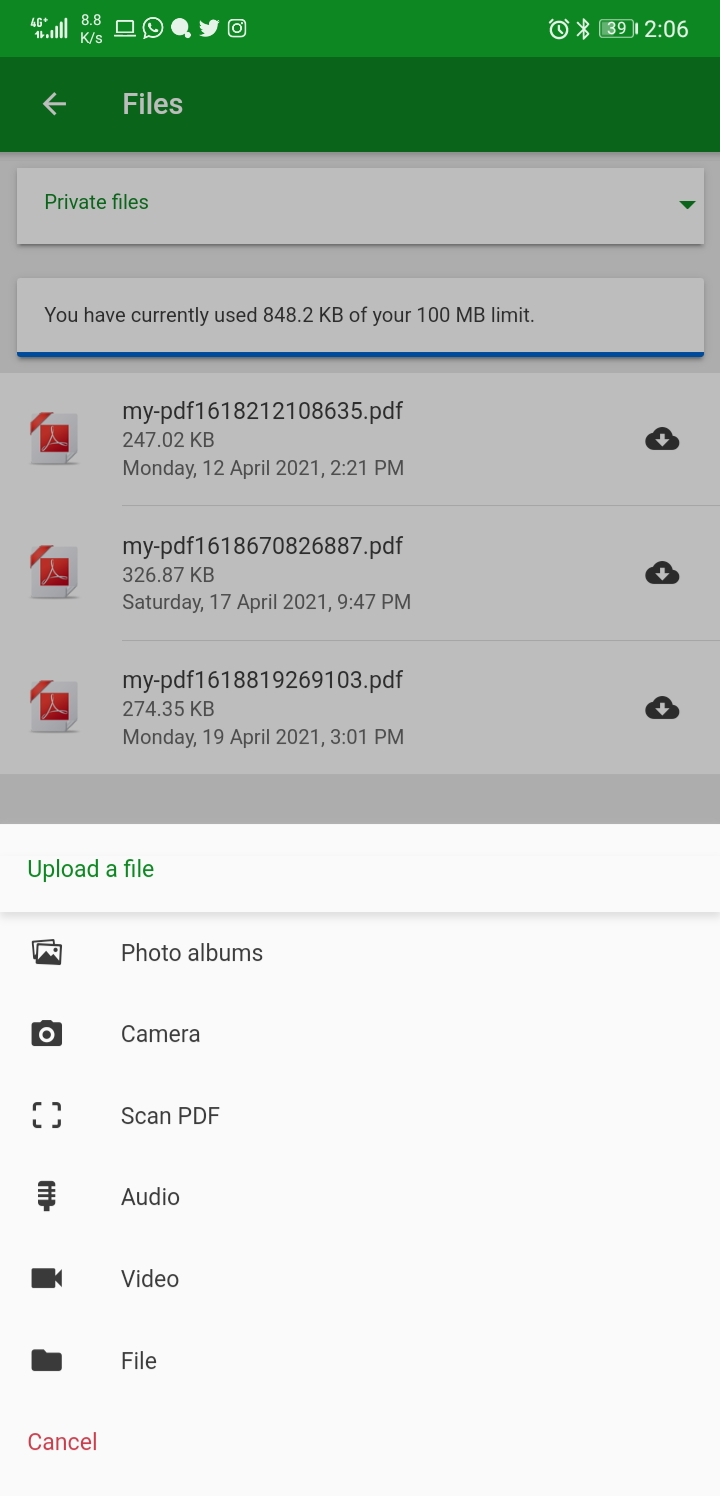
\includegraphics[scale=0.15]{scan-PDF-options_id.ac.unpar.moodlemobile.jpg}  
	\caption[Pilihan cara menggunggah file] {Pilihan cara menggunggah file} 
	\label{app:menu:files:options} 
\end{figure}  

Memilih pilihan \textit{Scan PDF} akan langsung mengarahkan pengguna ke kamera perangkat pengguna. Setelah pengguna mengambil gambar menggunakan kameranya. Pengguna akan diminta untuk menekan ikon tanda centang untuk mengkonfirmasi hasil pengambilan gambarnya, seperti pada Gambar \ref{app:scanPDF:confirm}.

\begin{figure}[H] 
	\centering  
	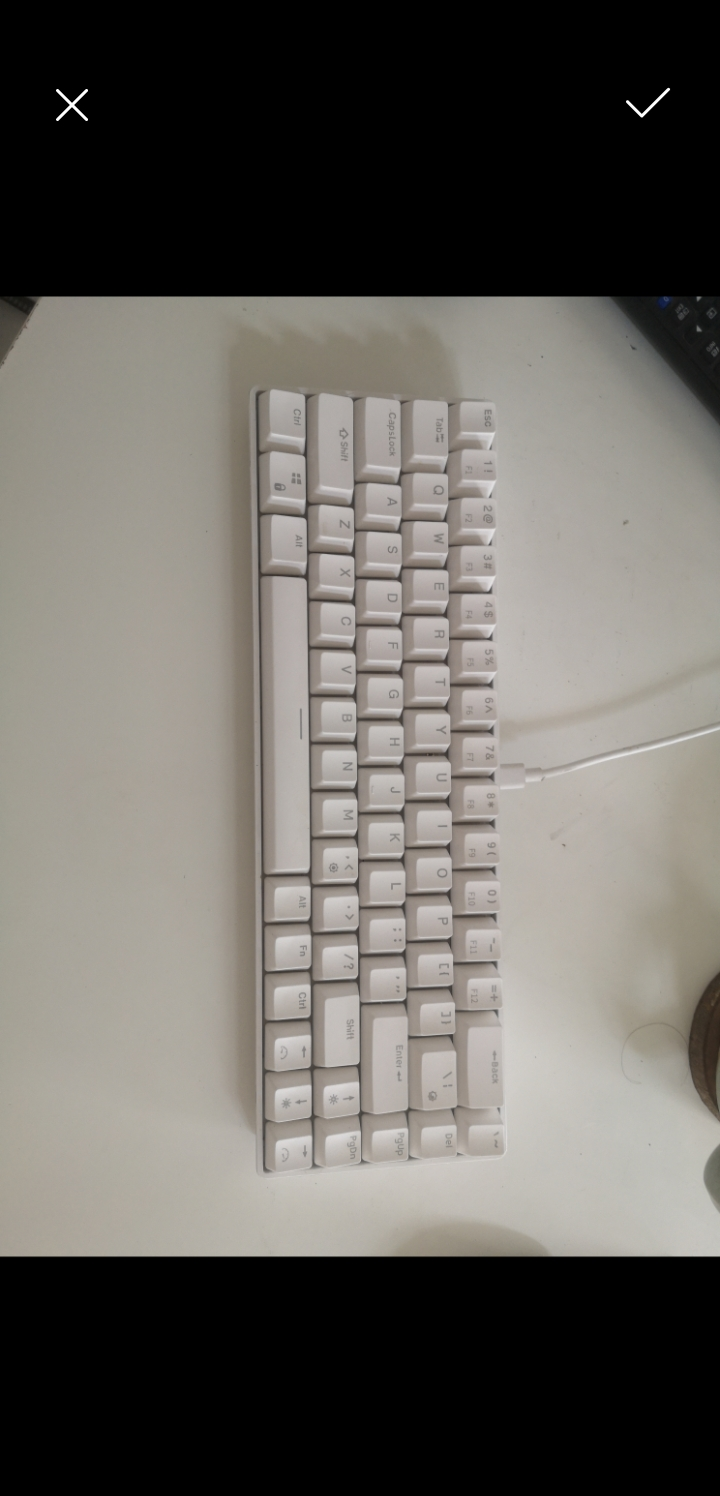
\includegraphics[scale=0.15]{scan-PDF-confirm_com.huawei.camera.jpg}  
	\caption[Konfirmasi hasil pengambilan gambar] {Konfirmasi hasil pengambilan gambar} 
	\label{app:scanPDF:confirm} 
\end{figure}  

Setelah mengkonfirmasi gambar yang telah diambil, aplikasi akan langsung memproses gambar menjadi sebuah file PDF. Pengguna akan mendapat konfirmasi kalau aplikasi telah berhasil memproses gambar dan mengunggahnya ke dalam \textit{private files} seperti pada Gambar \ref{app:scanPDF:success}. File yang akan dihasilakn akan diberi nama \texttt{my-pdf<date.getTime()>}. Untuk melihat file yang telah dihasilkan, pengguna harus mengunduhnya terlebih dahulu.

\begin{figure}[H] 
	\centering  
	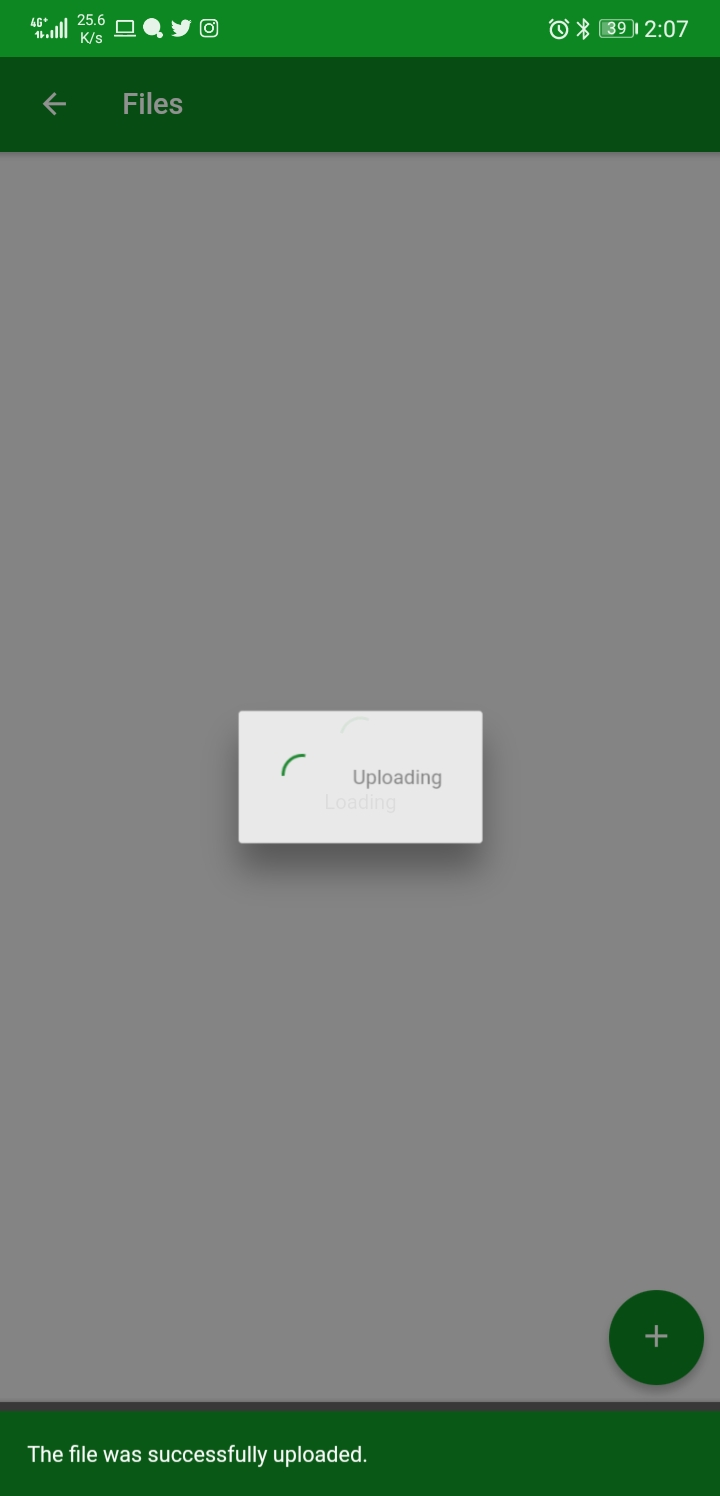
\includegraphics[scale=0.15]{scan-PDF-success_id.ac.unpar.moodlemobile.jpg}  
	\caption[Pemberitahuan bahwa file berhasil diproses dan diunggah] {Pemberitahuan bahwa file berhasil diproses dan diunggah} 
	\label{app:scanPDF:success} 
\end{figure}  

Pengguna juga dapat menggunakan fitur \textit{Scan PDF} untuk mengumpulkan tugas. Untuk melakukan hal tersebut, pengguna harus membuka tugas yang diinginkan seperti pada Gambar \ref{app:scanPDF:submission}. Kemudia menekan tombol \textit{ADD FILE} untuk memunculkan pilihan menggungah file seperti pada Gambar \ref{app:scanPDF:submission:options}. Setelah itu pengguna dapat menekan tombol \textit{save} untuk memfinalisasi submisi.

\begin{figure}[H]
	\centering
	\begin{minipage}{.3\textwidth}
	\centering  
	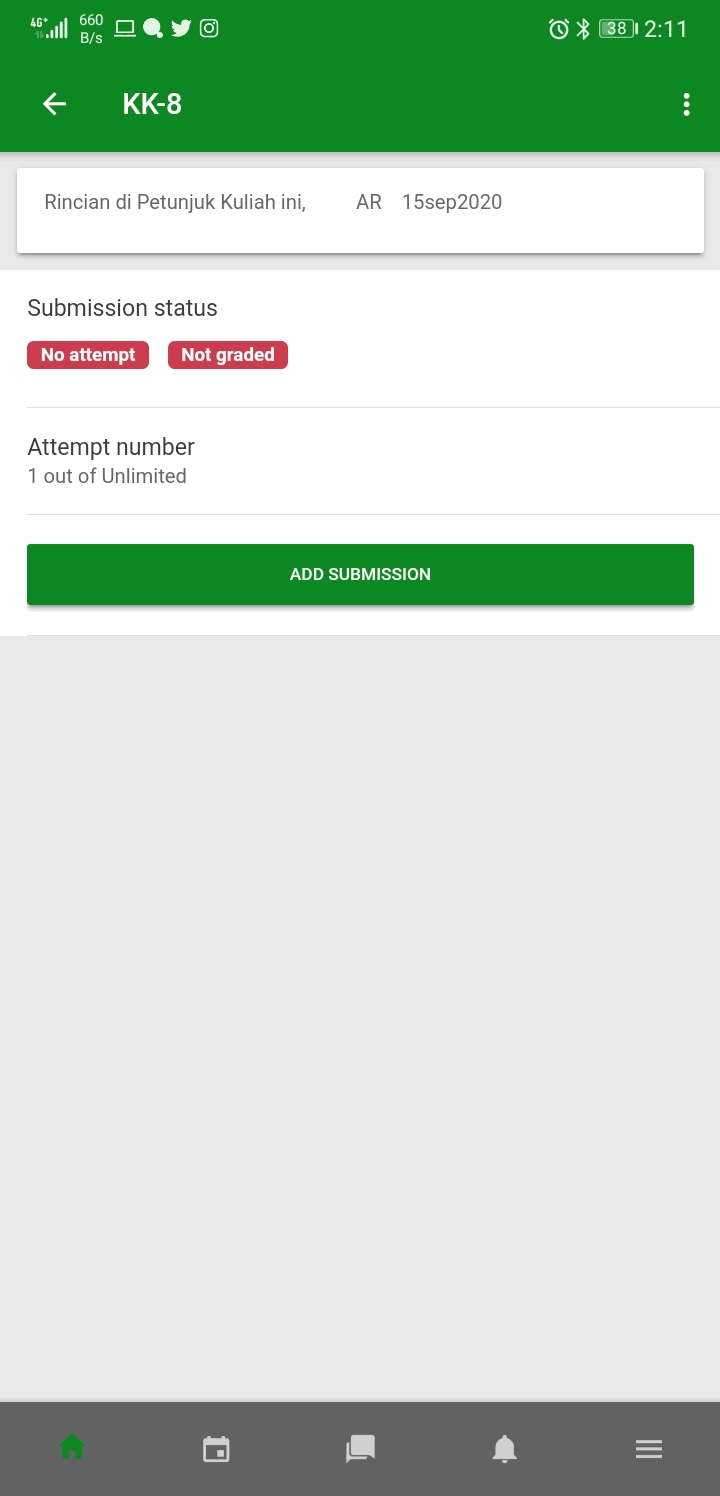
\includegraphics[scale=0.13]{scan-PDF-submission_id.ac.unpar.moodlemobile.jpg}  
	\caption[Halaman submisi tugas] {Halaman submisi tugas} 
	\label{app:scanPDF:submission} 
	\end{minipage}
	\hspace{.3\textwidth}
	\begin{minipage}{.3\textwidth}
	\centering  
	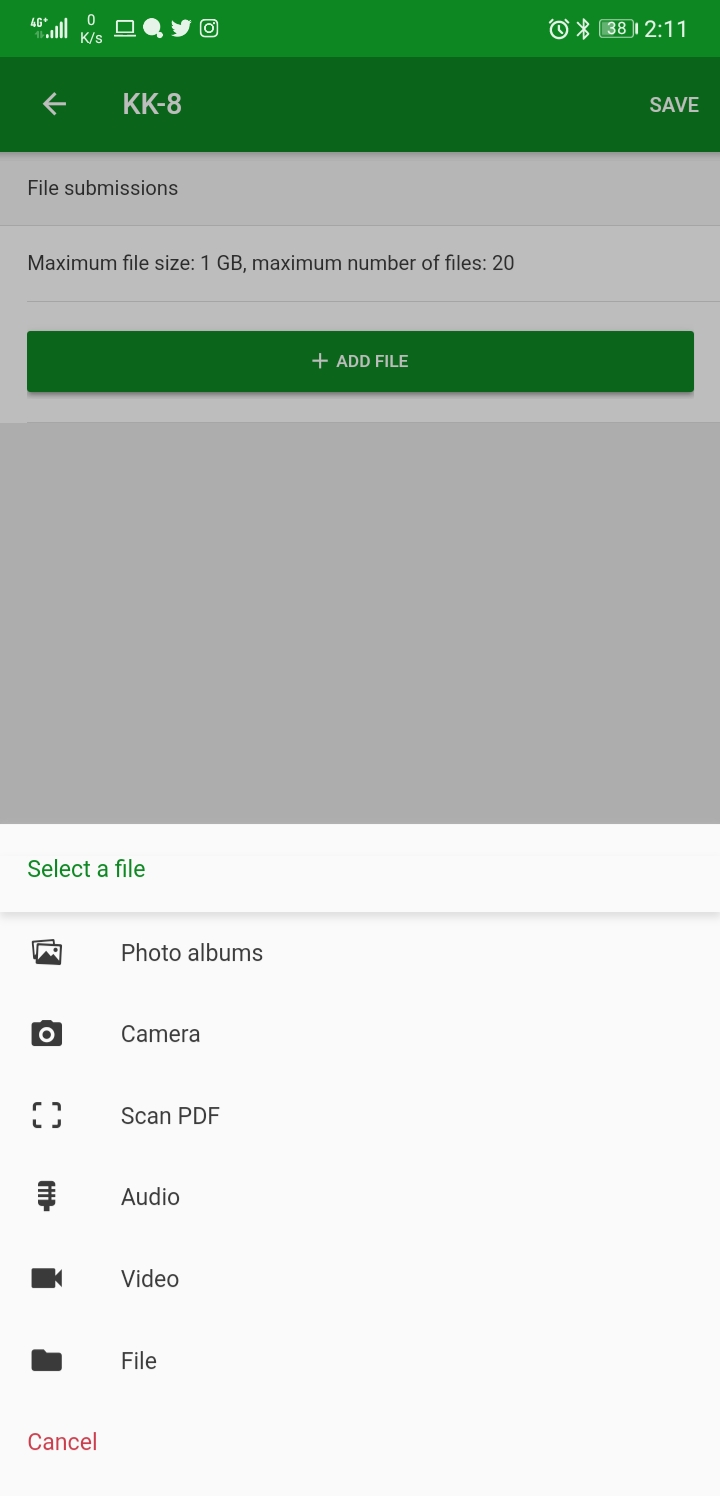
\includegraphics[scale=0.13]{scan-PDF-submission-options_id.ac.unpar.moodlemobile.jpg}  
	\caption[Pilihan submisi tugas] {Pilihan submisi tugas} 
	\label{app:scanPDF:submission:options} 
	\end{minipage}
\end{figure}

\subsection{Pengujian Eksperimental}

Pengujian eksperimental akan dilakukan dengan membagikan rilis terakhir aplikasi kepada mahasiswa UNPAR dan meminta mahasiswa untuk memberikan nilai 1 sampai 5 fitur \textit{files}, fitur mengumpulkan tugas, fitur messages, fitur \textit{Scan PDF}, dan fitur menu Student Portal. Selain memberikan nilai kepada fitur-fitur tersebut, mahasiswa juga dapat memberikan komentar tambahan mengenai penggunaan aplikasi IDE UNPAR mobile. Kuesioner mulai dibagikan pada tanggal 14 Juni 2021. 

Hasil dari pembagian kuesioner dapat dilihat sebagai berikut :

\begin{enumerate}
\item Kepuasan pengguji aplikasi terhadap fitur \textit{files} dapat dilihat pada Gambar \ref{responses:feature:files}. Dari gambar tersebut dapat diketahui bahwa mayoritas pengguna merasa puas dengan fitur \textit{files}. 
\begin{figure}[H] 
	\centering  
	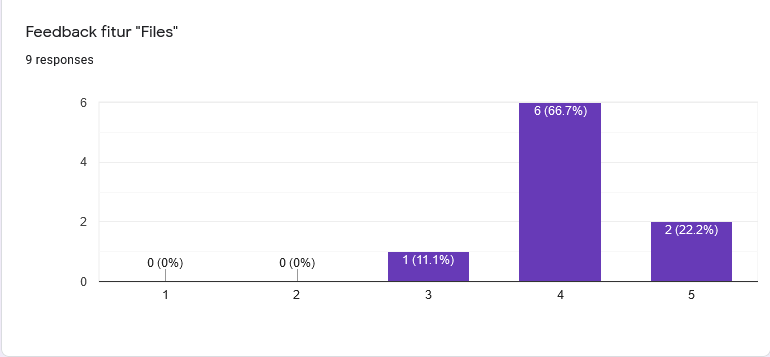
\includegraphics[scale=0.4]{form-fitur-files.png}  
	\caption[Kepuasan penguji terhadap fitur \textit{files}] {Kepuasan penguji terhadap fitur \textit{files}} 
	\label{responses:feature:files} 
\end{figure}

\item Kepuasan penguji terhadap fitur mengumpulkan tugas atau kuis dapat dilihat pada Gambar \ref{responses:feature:submission}. Dari gambar tersebut dapat diketahui bahwa mayoritas penguji merasa puas dengan fitur mengumpulkan tugas dan kuis.
\begin{figure}[H] 
	\centering  
	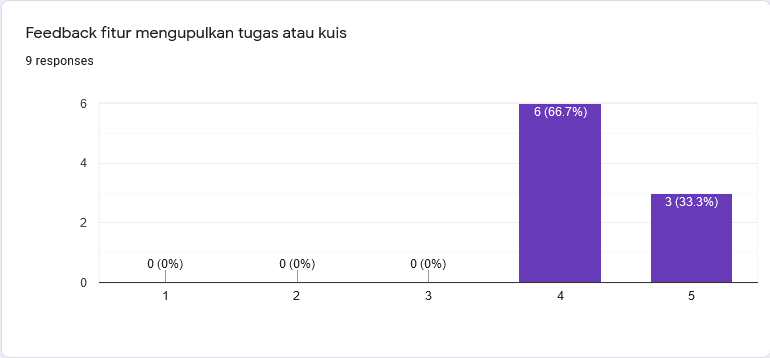
\includegraphics[scale=0.4]{form-fitur-tugas-dan-kuis.png}  
	\caption[Kepuasan penguji terhadap fitur mengumpulkan tugas dan kuis] {Kepuasan penguji terhadap fitur mengumpulkan tugas dan kuis} 
	\label{responses:feature:submission} 
\end{figure}

\item Kepuasan penguji terhadap fitur \textit{messages} dapat dilihat pada Gambar \ref{responses:feature:messages}. Dari gambar tersebut dapat diketahui bahwa mayoritas penguji merasa sangat puas dengan fitur \textit{messages}.
\begin{figure}[H] 
	\centering  
	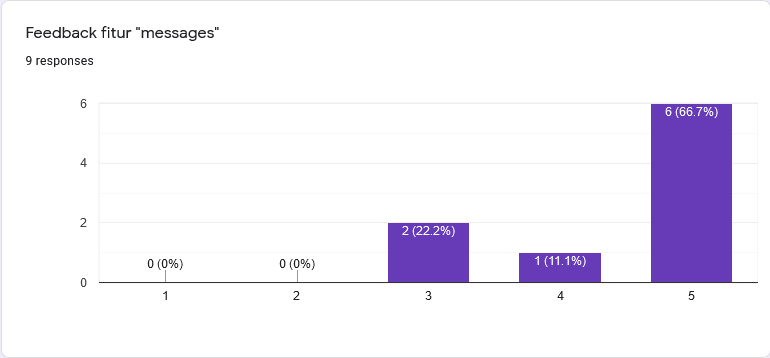
\includegraphics[scale=0.4]{form-fitur-messages.png}  
	\caption[Kepuasan penguji terhadap fitur \textit{messages}] {Kepuasan penguji terhadap fitur \textit{messages}} 
	\label{responses:feature:messages} 
\end{figure}

\item Kepuasan penguji terhadap fitur \textit{Scan PDF} dapat dilihat pada Gambar \ref{responses:feature:scanPDF}. Dari gambar tersebut dapat diketahui bahwa mayoritas penguji merasa sangat puas dengan fitur \textit{Scan PDF}.
\begin{figure}[H] 
	\centering  
	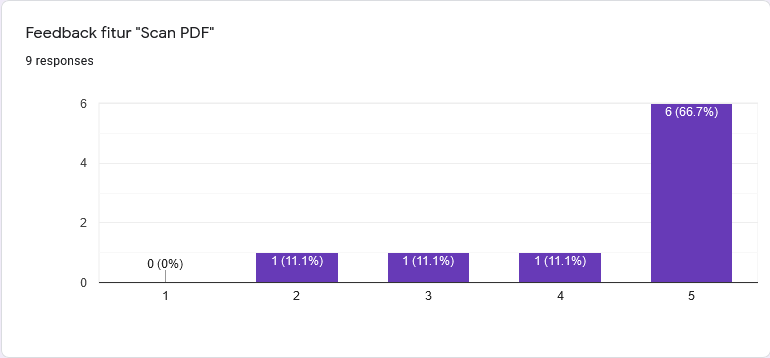
\includegraphics[scale=0.4]{form-fitur-scan-pdf.png}  
	\caption[Kepuasan penguji terhadap fitur \textit{Scan PDF}] {Kepuasan penguji terhadap fitur \textit{Scan PDF}} 
	\label{responses:feature:scanPDF} 
\end{figure}

\item Kepuasan penguji terhadap fitur menu Student Portal dapat dilihat pada Gambar \ref{responses:feature:stupor}. Dari gambar tersebut dapat diketahui bahwa mayoritas pengguna merasa sangat puas dengan fitur menu Student Portal.
\begin{figure}[H] 
	\centering  
	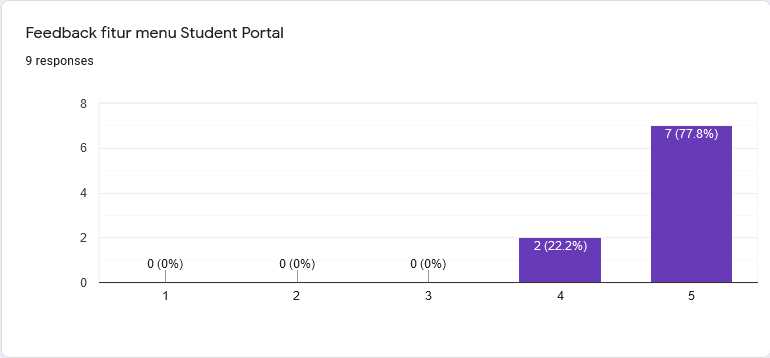
\includegraphics[scale=0.4]{form-fitur-student-portal.png}  
	\caption[Kepuasan penguji terhadap fitur menu Student Portal] {Kepuasan penguji terhadap fitur menu Student Portal} 
	\label{responses:feature:stupor} 
\end{figure}

\item Komentar tambahan yang diberikan oleh penguji dapat dilihat pada Tabel \ref{responses:comments}.

\begin{table}[ht]
\caption{Komentar-komentar yang diberikan oleh para penguji aplikasi}
\centering
\begin{tabular}{|l | l |}
\hline
\textbf{No} & \textbf{Komentar} \\  \hline
1 &  Tampilan masih sedikit membingungkan \\ \hline
2 & Aplikasi yang bagus untuk kelancaran kuliah \\ \hline
3 &  Saya tidak menemukan fitur \textit{logout} \\ 
\hline
\end{tabular}
\label{responses:comments}
\end{table}
	\begin{enumerate}
	\item \textbf{Tampilan masih sedikit membingungkan} \\
	Penyebab pengguna merasa tampilan masih membingungkan dimungkinkan karena, judul aplikasi pada halaman utama bertabrakan dengan ikon pencarian. Namun perbaikan tidak sempat diterapkan karena waktu yang tidak mencukupi.
	
	\item \textbf{Saya tidak menemukan fitur \textit{logout}} \\
	Fitur logout pada aplikasi IDE UNPAR mobile tidak terlabel sebagai \textit{logout}, melainkan menjadi \textit{Change site} seperti yang dibahas pada subbab \ref{pengujian:fungsional}.
	\end{enumerate}
\end{enumerate}



